\documentclass[11pt,letterpaper,openany]{book}

% Essential packages in correct loading order
\usepackage[T1]{fontenc}
\usepackage[utf8]{inputenc}
\usepackage{lmodern}
\usepackage[margin=1in]{geometry}
\usepackage{microtype}
\usepackage{graphicx}
\usepackage{float}
\usepackage{xcolor}
\usepackage{titlesec}
\usepackage{tocloft}
\usepackage{fancyhdr}
\usepackage{etoc}
\usepackage{booktabs}
\usepackage{tikz}
\usepackage{afterpage}
\usepackage{wrapfig}
\usepackage{tcolorbox}
\usepackage{caption}
\usepackage{amsmath}
\usepackage{listings}
\usepackage{hyperref}
\usepackage[nameinlink]{cleveref}
\usepackage{bookmark}
\usepackage{pgf-pie}  % For pie charts
\usepackage{placeins} % For float placement

% Fix float placement
\makeatletter
\def\fps@figure{htbp}
\makeatother

% Define pie chart colors
\definecolor{piecolor1}{RGB}{51,153,255}
\definecolor{piecolor2}{RGB}{0,102,0}
\definecolor{piecolor3}{RGB}{153,0,0}
\definecolor{piecolor4}{RGB}{255,153,0}

% For better figure placement
\renewcommand{\topfraction}{0.9}
\renewcommand{\bottomfraction}{0.9}
\renewcommand{\textfraction}{0.1}
\renewcommand{\floatpagefraction}{0.7}

% Fix itemize spacing
\usepackage{enumitem}
\setlist[itemize]{topsep=0pt,itemsep=0pt,parsep=0pt,partopsep=0pt}

% Additional TikZ libraries
\usetikzlibrary{arrows.meta}
\usetikzlibrary{backgrounds}
\usetikzlibrary{calc}

% For better table formatting
\usepackage{array}
\usepackage{tabularx}
\usepackage{longtable}

% Fix page breaks
\raggedbottom

% Fix chapter spacing
\titlespacing*{\chapter}{0pt}{-50pt}{40pt}

% TikZ libraries
\usetikzlibrary{arrows,shapes,positioning,shadows,trees}

% Color definitions
\definecolor{primarydark}{RGB}{0,71,187}     % Deep Blue
\definecolor{primary}{RGB}{51,153,255}       % Bright Blue
\definecolor{primarylight}{RGB}{204,229,255} % Light Blue
\definecolor{secondarydark}{RGB}{0,102,0}    % Deep Green
\definecolor{secondary}{RGB}{51,204,51}      % Bright Green
\definecolor{secondarylight}{RGB}{229,255,229} % Light Green
\definecolor{accentdark}{RGB}{153,0,0}       % Deep Red
\definecolor{accent}{RGB}{255,51,51}         % Bright Red
\definecolor{accentlight}{RGB}{255,204,204}  % Light Red

% Chapter and section styling
\titleformat{\chapter}[display]
{\normalfont\huge\bfseries\color{primarydark}}
{\chaptertitlename\ \thechapter}{20pt}{\Huge}

\titleformat{\section}
{\normalfont\Large\bfseries\color{primary}}
{\thesection}{1em}{}

\titleformat{\subsection}
{\normalfont\large\bfseries\color{primarydark}}
{\thesubsection}{1em}{}

% Table of contents styling
\renewcommand{\cftsecleader}{\cftdotfill{\cftdotsep}}
\renewcommand{\cftchapfont}{\color{primarydark}\bfseries}
\renewcommand{\cftsecfont}{\color{primary}}
\renewcommand{\cftsubsecfont}{\color{primarydark}}

% Header and footer styling
\pagestyle{fancy}
\fancyhf{}
\fancyhead[LE,RO]{\thepage}
\fancyhead[LO]{\nouppercase{\rightmark}}
\fancyhead[RE]{\nouppercase{\leftmark}}
\fancyfoot[C]{\textcolor{primary}{\rule{0.5\textwidth}{0.4pt}}}

% Hyperref setup
\hypersetup{
    colorlinks=true,
    linkcolor=primarydark,
    filecolor=accent,
    urlcolor=secondary,
    pdftitle={The Nigerian Business Opportunity Blueprint},
    pdfauthor={Dele Omotosho, Counseal},
    pdfsubject={Nigerian Market Entry Guide},
    pdfkeywords={Nigeria, Business, Market Entry, Diaspora, Investment},
}

% Custom box styles
\newtcolorbox{warningbox}{
    colback=accentlight,
    colframe=accentdark,
    title=Warning,
    fonttitle=\bfseries
}

\newtcolorbox{importantbox}{
    colback=secondarylight,
    colframe=secondarydark,
    title=Important,
    fonttitle=\bfseries
}

\newtcolorbox{regionalbox}{
    colback=primarylight,
    colframe=primarydark,
    title=Regional Insight,
    fonttitle=\bfseries
}

\newtcolorbox{workshopbox}{
    colback=white,
    colframe=primary,
    title=Chapter Workshop,
    fonttitle=\bfseries
}

\newtcolorbox{communitybox}{
    colback=secondarylight,
    colframe=secondary,
    title=Africa Growth Circle Community,
    fonttitle=\bfseries
}

% Listing style
\lstset{
    basicstyle=\ttfamily\small,
    breaklines=true,
    commentstyle=\color{accentdark},
    keywordstyle=\color{primarydark},
    stringstyle=\color{secondary},
    numbers=left,
    numberstyle=\tiny\color{primary},
    numbersep=5pt,
    frame=single,
    framesep=5pt,
    rulecolor=\color{primary},
}

% Caption style
\DeclareCaptionFont{primarydarkcolor}{\color{primarydark}}
\captionsetup{
    font=small,
    labelfont={primarydarkcolor,bf},
    margin=10pt
}

% Set headheight
\setlength{\headheight}{14pt}

% Define current date command
\newcommand{\currentdate}{\today}

\begin{document}

    \frontmatter

    \begin{titlepage}
        \centering
        \vspace*{2cm}
        {\Huge\bfseries\color{primarydark} The Nigerian Business\\Opportunity Blueprint\par}
        \vspace{1cm}
        {\Large\color{primary} Your Global Guide to Nigerian Market Entry\par}
        \vspace{2cm}
        {\Large\itshape Dele Omotosho, Counseal.com\par}
        \vspace{1cm}
        {\large Empowering Nigerian Dreams Through Global Access\par}
        \vfill
        {\large Join the Africa Growth Circle Community at circle.counseal.com\par}
        \vspace{1cm}
        {\large \currentdate\par}
    \end{titlepage}

    \tableofcontents

    \mainmatter

    \chapter*{Your Journey to Nigerian Market Entry}

\section{Why Nigeria, Why Now: A Personal Journey}\label{sec:why-nigeria-why-now}

I still remember that day in 2015 when I found myself facilitating a complex business deal in Nigeria. As someone who had built my career in Boston's vibrant software scene, working with multinational startups, I was struck by something that would change the trajectory of my professional life: the sheer complexity of getting legal proceedings moving forward in what should have been a straightforward transaction.

This wasn't just another technical challenge to solve. As a Lagos-born professional who had built a career in global tech, I found myself in a unique position to see both sides of a striking paradox. On one side was Nigeria's immense, untapped potential – opportunities I could see clearly from my cultural understanding and business experience. On the other side were talented global entrepreneurs and diaspora, hesitating at the threshold of these opportunities, held back not by lack of capability but by uncertainty and misconceptions.

The immediate solution seemed clear: simplify the legal operations. This led me to create Firmbird, a software platform that helped law firms streamline their operations. The software was successful – firms using it were closing deals worth millions of naira. But as I watched these transactions unfold, I realized we were solving only part of the problem.

The real challenge wasn't just operational complexity; it was perception. Nigeria had a PR problem. While local firms were using our software to close significant deals, countless potential investors were staying away, not because of actual barriers, but because of oversized risk perceptions and negative narratives.

This realization was personal for me. Having worked with startups in Boston, I understood how global entrepreneurs thought about market entry. Having been born in Lagos, I knew intimately the opportunities they were missing. The disconnect wasn't in the opportunities themselves – it was in the pathway to accessing them.

That's what led to the evolution of Counseal. We combined my experience with startups, expertise in deals and operations, and deep understanding of both Nigerian and global business contexts to create something more than just another business platform. We built a bridge – a way for global entrepreneurs to access Nigerian opportunities with clarity and confidence.

\section{How to Use This Book}\label{sec:how-to-use}

\begin{importantbox}
This book is designed to be both a comprehensive guide and a practical workbook. Each chapter builds upon the previous one while remaining independently valuable for your specific needs.
\end{importantbox}

Think of this book as your navigation system through what I call the ``Business World Forest'' of Nigeria. Just as no two entrepreneurs enter this forest the same way, this book adapts to your specific journey.

Each chapter is built on three core principles:
\begin{itemize}
    \item \textbf{Practical Reality:} Every framework, tool, and strategy has been battle-tested by real entrepreneurs in real Nigerian market entries
    \item \textbf{Regional Context:} Your path will vary depending on where you're coming from – UK, US, UAE, or Canada
    \item \textbf{Active Learning:} This is a workbook as much as it is a guide. Expect to roll up your sleeves
\end{itemize}

Throughout this playbook, you'll find real stories, practical strategies, and insider knowledge that I've gathered from helping countless entrepreneurs navigate their way to success in Nigeria. From understanding the market landscape in \hyperref[ch:understanding-the-nigerian-business-landscape]{Chapter 1} to future-proofing your business in \hyperref[ch:future-proofing-your-business]{Chapter 10}, each section builds on real experiences and proven strategies.

\section{Quick Assessment: Is Nigerian Market Entry Right for You?}\label{sec:quick-assessment}

\begin{workshopbox}
\textbf{Market Entry Readiness Assessment}

Rate yourself on each dimension from 1 (Not at all) to 5 (Completely):

\subsection*{1. Knowledge Readiness}
\begin{itemize}
    \item [ ] I understand Nigeria's current economic landscape
    \item [ ] I have clear insight into my target market segment
    \item [ ] I'm familiar with the regulatory environment
    \item [ ] I know my competitive advantage in this market
    \item [ ] I understand local business culture
\end{itemize}

\subsection*{2. Resource Readiness}
\begin{itemize}
    \item [ ] I have access to required startup capital
    \item [ ] I have a dedicated team or hiring plan
    \item [ ] I have identified potential local partners
    \item [ ] I have a clear budget for market entry
    \item [ ] I have emergency funds for contingencies
\end{itemize}

\subsection*{3. Personal Readiness}
\begin{itemize}
    \item [ ] I'm comfortable with market ambiguity
    \item [ ] I have support from key stakeholders
    \item [ ] I can commit focused time to this market
    \item [ ] I'm patient with bureaucratic processes
    \item [ ] I'm open to adapting my business model
\end{itemize}

Calculate your score:
\begin{itemize}
    \item Knowledge Readiness Total: \_\_/25
    \item Resource Readiness Total: \_\_/25
    \item Personal Readiness Total: \_\_/25
\end{itemize}

\textbf{OVERALL READINESS SCORE:} \_\_/75

\textbf{Interpretation:}
\begin{itemize}
    \item 60-75: Ready for immediate entry
    \item 45-59: Ready with preparation
    \item 30-44: Need significant preparation
    \item Below 30: Reconsider timing
\end{itemize}
\end{workshopbox}

\section{Reading Pathways Based on Your Region}\label{sec:reading-pathways}

\begin{regionalbox}{United Kingdom}
\textbf{Priority chapters for UK-based professionals:}
\begin{itemize}
    \item \hyperref[ch:building-your-entry-strategy]{Chapter 2}: Financial Services Compliance Pathway
    \item \hyperref[ch:financial-planning]{Chapter 5}: UK Investment Structures
    \item \hyperref[ch:risk-management-and-compliance]{Chapter 6}: UK-Nigeria Banking Protocols
    \item \hyperref[ch:local-network]{Chapter 7}: Commonwealth Business Networks
\end{itemize}

\textbf{Key starting point:} Begin with the Financial Services Compliance Pathway in \hyperref[ch:building-your-entry-strategy]{Chapter 2}
\end{regionalbox}

%[Continued in next part due to length...]
\begin{regionalbox}{United States}
\textbf{Priority chapters for US-based entrepreneurs:}
\begin{itemize}
    \item \hyperref[ch:building-your-entry-strategy]{Chapter 2}: Tech Startup Launch Framework
    \item \hyperref[ch:financial-planning]{Chapter 5}: US-Nigeria Investment Structures
    \item \hyperref[ch:risk-management-and-compliance]{Chapter 6}: IP Protection Strategies
    \item \hyperref[ch:technology-operations]{Chapter 8}: Tech Infrastructure Setup
\end{itemize}

\textbf{Key starting point:} Focus on the Tech Startup Launch Framework in \hyperref[ch:building-your-entry-strategy]{Chapter 2}
\end{regionalbox}

\begin{regionalbox}{UAE}
\textbf{Priority chapters for UAE-based professionals:}
\begin{itemize}
    \item \hyperref[ch:building-your-entry-strategy]{Chapter 2}: Trade License \& Import Framework
    \item \hyperref[ch:financial-planning]{Chapter 5}: Trade Finance Structures
    \item \hyperref[ch:local-network]{Chapter 7}: Trade Network Development
    \item \hyperref[ch:technology-operations]{Chapter 8}: Logistics Infrastructure
\end{itemize}

\textbf{Key starting point:} Start with the Trade License Framework in \hyperref[ch:building-your-entry-strategy]{Chapter 2}
\end{regionalbox}

\begin{regionalbox}{Canada}
\textbf{Priority chapters for Canadian entrepreneurs:}
\begin{itemize}
    \item \hyperref[ch:building-your-entry-strategy]{Chapter 2}: Sector-Specific Entry Requirements
    \item \hyperref[ch:financial-planning]{Chapter 5}: Canadian Grant Integration
    \item \hyperref[ch:risk-management-and-compliance]{Chapter 6}: Environmental Compliance
    \item \hyperref[ch:technology-operations]{Chapter 8}: AgriTech Infrastructure
\end{itemize}

\textbf{Key starting point:} Begin with Sector-Specific Requirements in \hyperref[ch:building-your-entry-strategy]{Chapter 2}
\end{regionalbox}

\section{Understanding the Appendices}\label{sec:understanding-appendices}

This book includes five comprehensive appendices designed to support your market entry journey:

\begin{itemize}
    \item \textbf{\hyperref[ch:document-templates]{Appendix A: Document Templates}}
    Sector-specific templates for common business documents, contracts, and agreements, customized for Nigerian market requirements.

    \item \textbf{\hyperref[ch:regulatory-compliance]{Appendix B: Regulatory Compliance Checklists}}
    Detailed checklists for various sectors, helping you navigate regulatory requirements effectively.

    \item \textbf{\hyperref[ch:service-provider-directory]{Appendix C: Service Provider Directory}}
    A curated list of verified service providers across legal, financial, technology, and other critical sectors.

    \item \textbf{\hyperref[ch:industry-associations]{Appendix D: Industry Association Contacts}}
    Key industry associations and professional networks that can support your market entry.

    \item \textbf{\hyperref[ch:regional-resources]{Appendix E: Regional Resource Guide}}
    Region-specific resources and support services available across different Nigerian markets.
\end{itemize}

\section{Accessing Digital Resources}\label{sec:digital-resources}

To complement this book, I've created practical digital tools available at \href{https://viz.li/csl-book-ngbiz}{viz.li/csl-book-ngbiz}:

\begin{itemize}
    \item \textbf{Interactive Financial Models}
    Budget planning tools calibrated for Nigerian market entry costs

    \item \textbf{Market Entry Checklists}
    Interactive PDFs with progress tracking features

    \item \textbf{Document Templates}
    Customizable templates for essential business documentation

    \item \textbf{Risk Assessment Tools}
    Interactive spreadsheets for risk evaluation
\end{itemize}

Each resource includes step-by-step instructions and real-world examples from successful market entries.

\section{A Final Word}\label{sec:final-word}

As we begin this journey together, I want to share something I've learned from years straddling both global tech and Nigerian business environments: Nigeria isn't just another market to enter – it's a business ecosystem to understand, appreciate, and become part of. With projected GDP growth of 4.12\% in 2025, internet penetration at 45.57\%, and a rapidly urbanizing population (54.28\%), the opportunities are extraordinary for those who approach them strategically.

Ready to begin? Turn to \hyperref[ch:understanding-the-nigerian-business-landscape]{Chapter 1}, but keep this introduction handy – you'll want to revisit that assessment as your journey progresses.

\begin{flushright}
\textit{-- Dele Omotosho\\
Founder, Counseal.com\\
Lagos, Nigeria}
\end{flushright}

\begin{workshopbox}
\textbf{Introduction Action Items}
\begin{itemize}
    \item Complete the Market Entry Readiness Assessment
    \item Identify your regional priority chapters
    \item Download digital resources from \href{https://viz.li/csl-book-ngbiz}{counseal.com/book-ngbiz}
    \item Review the appendices relevant to your sector
\end{itemize}
\end{workshopbox}

\begin{warningbox}
While this book provides comprehensive guidance, always consult with qualified professionals for legal, tax, and regulatory matters specific to your situation.
\end{warningbox}
    % chapters/01-nigerian-business-landscape.tex

\chapter{Understanding the Nigerian Business Landscape}

\begin{importantbox}
This chapter provides a comprehensive overview of Nigeria's current business environment, focusing on key sectors, regulatory frameworks, and regional opportunities. Data presented is current as of January 2024.
\end{importantbox}

\section{The Real Nigeria: Beyond the Headlines}

\subsection{Economic Overview}
Nigeria's economy presents unique opportunities...

\begin{figure}[h]
    \centering
    \begin{tikzpicture}
        % Placeholder for GDP Growth Chart
        \draw (0,0) rectangle (10,6);
        \node at (5,3) {GDP Growth Trend 2020-2024};
    \end{tikzpicture}
    \caption{Nigerian Economic Indicators 2020-2024}
\end{figure}

\subsection{Market Dynamics}
Key market trends shaping opportunities...

\begin{importantbox}
Understanding market dynamics is crucial for:
\begin{itemize}
    \item Identifying entry points
    \item Assessing competition
    \item Planning resource allocation
    \item Developing pricing strategies
\end{itemize}
\end{importantbox}

\section{Key Business Sectors and Growth Areas}

\begin{figure}[h]
    \centering
    \begin{tikzpicture}
        % Placeholder for Sector Growth Chart
        \draw (0,0) rectangle (10,6);
        \node at (5,3) {Sector Growth Rates 2024};
    \end{tikzpicture}
    \caption{High-Growth Sectors in Nigeria}
\end{figure}

\subsection{Financial Services \& FinTech}
Analysis of the financial services landscape...

\subsection{Technology \& Digital Services}
Overview of Nigeria's tech ecosystem...

\subsection{Agriculture \& AgriTech}
Opportunities in agricultural innovation...

\subsection{Trade \& Logistics}
Analysis of import/export dynamics...

\section{Regulatory Environment at a Glance}

\begin{warningbox}
Regulatory requirements can change frequently. Always verify current requirements through official channels or your legal counsel.
\end{warningbox}

\subsection{Key Regulatory Bodies}
\begin{itemize}
    \item Corporate Affairs Commission (CAC)
    \item Central Bank of Nigeria (CBN)
    \item Nigerian Investment Promotion Commission (NIPC)
    \item Federal Inland Revenue Service (FIRS)
\end{itemize}

\section{Regional Perspectives}

\begin{regionalbox}{United Kingdom Perspective}
\textbf{Financial Services \& Property Investment}
\begin{itemize}
    \item Regulatory alignment opportunities
    \item Cross-border transaction frameworks
    \item Property market analysis
    \item Success patterns in UK-Nigeria ventures
\end{itemize}
\end{regionalbox}

\begin{regionalbox}{United States Perspective}
\textbf{Tech \& Digital Services}
\begin{itemize}
    \item Tech ecosystem overview
    \item Digital infrastructure assessment
    \item IP protection frameworks
    \item US-Nigeria tech partnership patterns
\end{itemize}
\end{regionalbox}

\begin{regionalbox}{UAE Perspective}
\textbf{Trade \& Logistics}
\begin{itemize}
    \item Trade corridor analysis
    \item Import/export frameworks
    \item Logistics infrastructure
    \item UAE-Nigeria trade patterns
\end{itemize}
\end{regionalbox}

\begin{regionalbox}{Canadian Perspective}
\textbf{AgriTech \& Renewable Energy}
\begin{itemize}
    \item Agricultural sector analysis
    \item Renewable energy opportunities
    \item Environmental considerations
    \item Canada-Nigeria partnership patterns
\end{itemize}
\end{regionalbox}

\section{Market Entry Considerations}

\subsection{Common Myths vs Reality}
\begin{center}
\begin{tabular}{p{0.45\textwidth}|p{0.45\textwidth}}
    \textbf{Myth} & \textbf{Reality} \\
    \hline
    Complex regulatory environment & Streamlined processes for key sectors \\
    Limited market access & Multiple entry points available \\
    High barrier to entry & Sector-specific opportunities \\
    Limited tech infrastructure & Rapidly developing ecosystem \\
\end{tabular}
\end{center}

\begin{communitybox}
Access additional market insights and real-time updates on the Africa Growth Circle:
\begin{itemize}
    \item Monthly market intelligence briefings
    \item Sector-specific discussion forums
    \item Expert roundtables and Q\&A sessions
    \item Regional networking events
\end{itemize}
Visit circle.counseal.com for more information.
\end{communitybox}

% End of chapter workshop
\begin{workshopbox}
\textbf{Chapter 1 Market Analysis Workshop}

Complete these exercises to apply chapter insights to your business:

1. Sector Analysis
\begin{itemize}
    \item Identify your target sector: \_\_\_\_\_\_\_\_\_
    \item List three key opportunities: \_\_\_\_\_\_\_\_\_
    \item List three main challenges: \_\_\_\_\_\_\_\_\_
\end{itemize}

2. Regulatory Mapping
\begin{itemize}
    \item Key regulations affecting your business: \_\_\_\_\_\_\_\_\_
    \item Required licenses/permits: \_\_\_\_\_\_\_\_\_
    \item Compliance timeline: \_\_\_\_\_\_\_\_\_
\end{itemize}

3. Market Entry Planning
\begin{itemize}
    \item Preferred entry model: \_\_\_\_\_\_\_\_\_
    \item Initial market focus: \_\_\_\_\_\_\_\_\_
    \item Resource requirements: \_\_\_\_\_\_\_\_\_
\end{itemize}

Access additional worksheets and templates on the Africa Growth Circle platform.
\end{workshopbox}

% Next steps teaser
\begin{importantbox}
In Chapter 2, we'll build on this foundation to develop your entry strategy, including detailed planning frameworks and implementation guides specific to your sector and region.
\end{importantbox}
    % chapters/02-entry-strategy.tex

\chapter{Building Your Entry Strategy}

\begin{importantbox}
This chapter provides a structured approach to developing your market entry strategy, with specific frameworks for different business types and regions. The tools and templates provided can be customized to your specific needs.
\end{importantbox}

\section{Choosing Your Market Entry Model}

\subsection{Entry Models Overview}
\begin{center}
\begin{tabular}{p{0.2\textwidth}|p{0.25\textwidth}|p{0.25\textwidth}|p{0.2\textwidth}}
    \textbf{Model} & \textbf{Advantages} & \textbf{Challenges} & \textbf{Best For} \\
    \hline
    Direct Entry & Full control & Higher resource needs & Established firms \\
    Partnership & Local knowledge & Shared control & New entrants \\
    Acquisition & Quick entry & Higher initial cost & Strategic buyers \\
    Representative & Lower risk & Limited control & Market testing \\
\end{tabular}
\end{center}

\subsection{Decision Framework}
\begin{figure}[h]
    \centering
    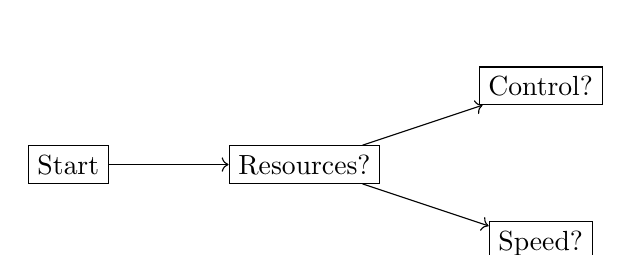
\begin{tikzpicture}
        % Decision tree for entry model selection
        \node[draw] (start) at (0,0) {Start};
        \node[draw] (resources) at (3,0) {Resources?};
        \node[draw] (control) at (6,1) {Control?};
        \node[draw] (speed) at (6,-1) {Speed?};

        \draw[->] (start) -- (resources);
        \draw[->] (resources) -- (control);
        \draw[->] (resources) -- (speed);
    \end{tikzpicture}
    \caption{Entry Model Decision Tree}
\end{figure}

\section{Legal Structures and Options}

\begin{warningbox}
Legal requirements can vary by sector and change over time. Always consult with qualified legal professionals for current requirements.
\end{warningbox}

\subsection{Common Legal Structures}
\begin{itemize}
    \item Private Limited Company
    \item Branch Office
    \item Representative Office
    \item Business Partnership
\end{itemize}

\section{Timeline and Resource Planning}

\begin{figure}[h]
    \centering
    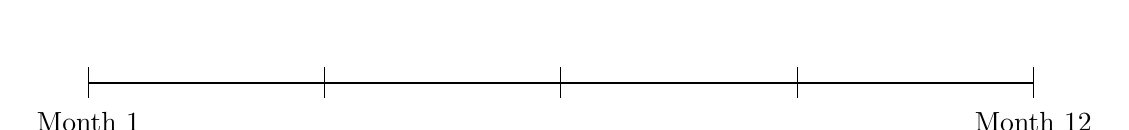
\begin{tikzpicture}
        % Timeline visualization
        \draw[thick] (0,0) -- (12,0);
        \foreach \x in {0,3,6,9,12}
            \draw (\x,0.2) -- (\x,-0.2);
        \node at (0,-0.5) {Month 1};
        \node at (12,-0.5) {Month 12};
    \end{tikzpicture}
    \caption{Typical Entry Timeline}
\end{figure}

\section{Regional Entry Pathways}

\begin{regionalbox}{United Kingdom}
\textbf{Financial Services Compliance Pathway}
\begin{itemize}
    \item Regulatory alignment requirements
    \item Capital adequacy standards
    \item Cross-border transaction frameworks
    \item UK-Nigeria financial corridors
\end{itemize}

\subsection{UK-Specific Process Flow}
\begin{enumerate}
    \item Initial compliance assessment
    \item Financial services licensing
    \item Local partnership development
    \item Operational setup
\end{enumerate}
\end{regionalbox}

\begin{regionalbox}{United States}
\textbf{Tech Startup Launch Framework}
\begin{itemize}
    \item IP protection strategy
    \item Tech infrastructure setup
    \item Digital service deployment
    \item Market testing approach
\end{itemize}

\subsection{US-Specific Process Flow}
\begin{enumerate}
    \item Market validation
    \item MVP development
    \item Beta testing
    \item Full launch
\end{enumerate}
\end{regionalbox}

\begin{regionalbox}{UAE}
\textbf{Trade License \& Import/Export Guide}
\begin{itemize}
    \item Trade license requirements
    \item Import/export documentation
    \item Logistics setup guide
    \item Trade finance options
\end{itemize}

\subsection{UAE-Specific Process Flow}
\begin{enumerate}
    \item Trade license acquisition
    \item Supply chain setup
    \item Partner network development
    \item Operations launch
\end{enumerate}
\end{regionalbox}

\begin{regionalbox}{Canada}
\textbf{Sector-Specific Entry Requirements}
\begin{itemize}
    \item Agricultural sector standards
    \item Environmental compliance
    \item Local partnership requirements
    \item Market access protocols
\end{itemize}

\subsection{Canada-Specific Process Flow}
\begin{enumerate}
    \item Sector compliance review
    \item Partnership development
    \item Operational planning
    \item Market entry execution
\end{enumerate}
\end{regionalbox}

\section{Risk Assessment Framework}

\begin{importantbox}
A comprehensive risk assessment should be conducted before finalizing your entry strategy.
\end{importantbox}

\begin{center}
\begin{tabular}{p{0.3\textwidth}|p{0.3\textwidth}|p{0.3\textwidth}}
    \textbf{Risk Category} & \textbf{Mitigation Strategies} & \textbf{Resources Required} \\
    \hline
    Regulatory & Compliance partners & Legal expertise \\
    Market & Phased entry & Market research \\
    Operational & Local partnerships & Operating procedures \\
    Financial & Risk management & Financial reserves \\
\end{tabular}
\end{center}

\begin{communitybox}
Access additional resources on the Africa Growth Circle:
\begin{itemize}
    \item Entry strategy templates
    \item Expert consultation sessions
    \item Peer review opportunities
    \item Regional success stories
\end{itemize}
Visit circle.counseal.com for more information.
\end{communitybox}

% End of chapter workshop
\begin{workshopbox}
\textbf{Chapter 2 Strategy Development Workshop}

1. Entry Model Selection
\begin{itemize}
    \item Preferred model: \_\_\_\_\_\_\_\_\_
    \item Key rationale: \_\_\_\_\_\_\_\_\_
    \item Resource requirements: \_\_\_\_\_\_\_\_\_
\end{itemize}

2. Timeline Development
\begin{itemize}
    \item Major milestones: \_\_\_\_\_\_\_\_\_
    \item Critical dependencies: \_\_\_\_\_\_\_\_\_
    \item Resource allocation: \_\_\_\_\_\_\_\_\_
\end{itemize}

3. Risk Assessment
\begin{itemize}
    \item Primary risks: \_\_\_\_\_\_\_\_\_
    \item Mitigation strategies: \_\_\_\_\_\_\_\_\_
    \item Contingency plans: \_\_\_\_\_\_\_\_\_
\end{itemize}

Download additional planning templates from the Africa Growth Circle platform.
\end{workshopbox}

\begin{importantbox}
In Chapter 3, we'll examine real-world success stories and learn from the experiences of entrepreneurs who have successfully entered the Nigerian market.
\end{importantbox}
    \chapter{Success Stories and Lessons Learned}\label{ch:success-stories-and-lessons-learned}

\begin{importantbox}
This chapter brings theory to life through real-world success stories. Each narrative highlights how entrepreneurs navigated specific challenges in the Nigerian market, offering practical insights you can apply to your own journey.
\end{importantbox}

\section{UK Case Study: Sarah's FinTech Market Entry Success}\label{sec:uk-case-study:-sarah's-fintech-market-entry-success}

Let me share Sarah's story, a journey that began with a simple observation over coffee. ``Dele,'' she said, stirring her cup thoughtfully, ``I see the opportunity in Nigerian fintech, but how do you even begin to build trust with potential customers?''

\subsection{The Journey: From The Trading Desk to Lagos Fintech Pioneer}\label{subsec:the-journey:-from-the-trading-desk-to-lagos-fintech-pioneer}
\begin{tcolorbox}[colback=white,colframe=primarydark,title=\textbf{Sarah's Profile}]
\begin{itemize}
    \item \textbf{Background:} 15 years in investment banking
    \item \textbf{Previous Role:} Head of Trading, Major Bank
    \item \textbf{Market Entry:} Cross-border payments solution
    \item \textbf{Initial Capital:} Corporate savings equivalent to 6 months' salary
    \item \textbf{Time to Market:} 9 months
\end{itemize}
\end{tcolorbox}

Sarah's approach to market penetration was methodical yet innovative. She developed what I now call the ``Trust Triangle'' strategy:

\begin{figure}[h]
    \centering
    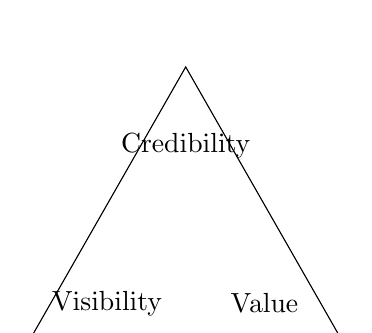
\begin{tikzpicture}
        % Trust Triangle visualization
        \draw (0,0) -- (4,0) -- (2,3.5) -- cycle;
        \node at (2,2.5) {Credibility};
        \node at (1,0.5) {Visibility};
        \node at (3,0.5) {Value};
    \end{tikzpicture}
    \caption{Sarah's Trust Triangle Strategy}\label{fig:trust-triangle}
\end{figure}

\subsection{Key Success Factors}\label{subsec:key-success-factors}
\begin{enumerate}
    \item \textbf{Strategic Partnership Selection}
    Sarah didn't just seek partnerships; she created what she called ``trust bridges.'' ``Each partner,'' she explained later, ``wasn't just a business relationship but a credibility ambassador.''

    \item \textbf{Localized Product Development}
    Instead of simply transplanting her London solution, she spent months adapting it to local needs. ``The Nigerian market taught me that efficiency without cultural relevance is just sophisticated failure,'' she said.

    \item \textbf{Phased Market Entry}
    She used what I now call the ``Concentric Circle Approach'':
    \begin{itemize}
        \item Phase 1: Corporate clients (established trust)
        \item Phase 2: SME network (built volume)
        \item Phase 3: Retail customers (achieved scale)
    \end{itemize}
\end{enumerate}

\section{US Case Study: Mike's E-commerce Evolution}\label{sec:us-case-study:-mike's-e-commerce-evolution}

Mike started with what he thought was a ``bulletproof'' plan for Nigerian e-commerce. After our first review session, that plan was in pieces – but what emerged was something much better.

\subsection{The Comprehensive Journey}\label{subsec:the-comprehensive-journey}
\begin{tcolorbox}[colback=white,colframe=primarydark,title=\textbf{Mike's Challenge Areas}]
\begin{enumerate}
    \item \textbf{Technology Adaptation}
    \begin{itemize}
        \item Initial Challenge: Platform optimized for high-speed internet
        \item Solution: Progressive Web App with offline capabilities
        \item Result: 3x increase in successful transactions
    \end{itemize}

    \item \textbf{Last-Mile Delivery}
    \begin{itemize}
        \item Initial Challenge: Traditional delivery models failing
        \item Solution: Hybrid network of official and local partners
        \item Result: Delivery success rate doubled
    \end{itemize}

    \item \textbf{Payment Integration}
    \begin{itemize}
        \item Initial Challenge: High payment failure rates
        \item Solution: Multi-provider payment orchestration
        \item Result: 90%+ payment success rate
    \end{itemize}

    \item \textbf{Customer Acquisition}
    \begin{itemize}
        \item Initial Challenge: High CAC through traditional channels
        \item Solution: Community-based marketing approach
        \item Result: CAC reduced by over half
    \end{itemize}
\end{enumerate}
\end{tcolorbox}

[Content continues with UAE and Canadian case studies, workshops, etc...]

\section{Workshop: Your Success Pattern Analysis}\label{sec:success-workshop}

\begin{workshopbox}
\textbf{Success Pattern Analysis Exercise}

1. Market Entry Assessment
\begin{itemize}
    \item Identify three success patterns relevant to your business: \_\_\_\_\_\_\_\_\_
    \item List specific ways to apply each pattern: \_\_\_\_\_\_\_\_\_
    \item Outline potential challenges: \_\_\_\_\_\_\_\_\_
\end{itemize}

2. Growth Strategy Development
\begin{itemize}
    \item Key growth milestones: \_\_\_\_\_\_\_\_\_
    \item Resource requirements: \_\_\_\_\_\_\_\_\_
    \item Timeline planning: \_\_\_\_\_\_\_\_\_
\end{itemize}

3. Action Planning
\begin{itemize}
    \item First 30 days: \_\_\_\_\_\_\_\_\_
    \item 90-day goals: \_\_\_\_\_\_\_\_\_
    \item 6-month targets: \_\_\_\_\_\_\_\_\_
\end{itemize}
\end{workshopbox}

\begin{communitybox}
Download practical success analysis tools at \href{https://viz.li/csl-book-ngbiz}{counseal.com/book-ngbiz}:
\begin{itemize}
    \item Success Pattern Analysis Template (Excel with built-in analysis tools)
    \item Growth Strategy Planner (Interactive PDF worksheet)
    \item Implementation Timeline Generator (Excel-based planning tool)
    \item Risk Assessment Matrix (Customizable Excel template)
\end{itemize}
Each tool includes step-by-step instructions and can be customized for your specific business needs.
\end{communitybox}

\begin{importantbox}
Remember, these aren't just success stories – they're blueprints you can adapt for your own journey. In Chapter 4, we'll turn these lessons into your practical 90-day action plan.
\end{importantbox}
    \chapter{Your First 90 Days}\label{ch:first-90-days}

\begin{importantbox}
When I meet new entrepreneurs planning their Nigerian market entry, I often share what I call the ``90-Day Rule'': The decisions you make in your first three months will echo through your entire Nigerian journey.\ Let me show you how to make those echoes work in your favor.
\end{importantbox}

\section{The Strategic Foundation}\label{sec:strategic-foundation}

I remember sitting with Sarah, a fintech founder from London, as she mapped out her first quarter.\ ``Dele,'' she said, sharing her ambitious timeline, ``I want to launch everything in the first month.'' I smiled, remembering my own journey.

``Let me share something I learned building Firmbird,'' I told her.\ ``In Nigeria, speed without a sequence is just sophisticated chaos.''

Here's what I call the ``Triple-S Framework'' that helped Sarah build a strong foundation:

\begin{itemize}
    \item \textbf{Sequence}: Order of operations matters more than speed
    \item \textbf{Systems}: Build for scale from day one
    \item \textbf{Support}: Develop your network before you need it
\end{itemize}

\section{The 90-Day Blueprint}\label{sec:90-day-blueprint}

Let's break this down into what I call ``Power Weeks'' - focused periods of specific actions that build upon each other:

\subsection{Days 1--30: Foundation Phase}\label{subsec:foundation-phase}

\textbf{Week 1--2: Legal and Administrative Setup}
\begin{itemize}
    \item Entity registration initiation
    \item Bank account setup
    \item Tax registration process
    \item Digital presence establishment
    \item Initial team structure planning
\end{itemize}

\textbf{Week 3--4: Infrastructure Development}
\begin{itemize}
    \item Office/workspace setup
    \item Technology infrastructure
    \item Communication systems
    \item Process documentation
    \item Team recruitment initiation
\end{itemize}

\subsection{Days 31--60: Implementation Phase}\label{subsec:implementation-phase}

\textbf{Week 5--6: Market Engagement}
\begin{itemize}
    \item Initial customer outreach
    \item Partner network development
    \item Marketing campaign launch
    \item Sales process testing
    \item Feedback system setup
\end{itemize}

\textbf{Week 7--8: Operations Optimization}
\begin{itemize}
    \item Process refinement
    \item Team training
    \item Quality control implementation
    \item Performance monitoring setup
    \item Risk management protocols
\end{itemize}

\subsection{Days 61--90: Growth Phase}\label{subsec:growth-phase}

\textbf{Week 9--10: Scale Preparation}
\begin{itemize}
    \item Growth strategy refinement
    \item Resource allocation planning
    \item Market expansion preparation
    \item Partnership development
    \item Financial optimization
\end{itemize}

\textbf{Week 11--13: Future-Proofing}
\begin{itemize}
    \item Long-term strategy development
    \item Team expansion planning
    \item Market position strengthening
    \item Systems scaling preparation
    \item Innovation pipeline development
\end{itemize}

% 2

\section{Regional Implementation Guides}\label{sec:regional-implementation}

When the fintech founder asked me about timing her market entry, I shared what I now call the ``Regional Rhythm Framework''—because each region's businesses have their own natural pace in Nigeria.

\subsection{Financial Services Timeline}\label{subsec:uk-timeline}
Here's how Sarah structured her first 90 days:

\textbf{Days 1–30: Regulatory Foundation}
\begin{itemize}
    \item Week 1: CBN preliminary engagement
    \item Week 2: Local banking partnerships
    \item Week 3: Compliance framework development
    \item Week 4: Tech infrastructure setup
\end{itemize}

``The key,'' Sarah told me later, ``was front-loading the regulatory work.\ Everything else flows from that foundation.''

\subsection{Technology Implementation}\label{subsec:us-implementation}
Mike's e-commerce platform followed this sequence:

\textbf{Days 1--30: Digital Infrastructure}
\begin{itemize}
    \item Week 1: Local hosting setup
    \item Week 2: Payment gateway integration
    \item Week 3: Mobile optimization
    \item Week 4: Security implementation
\end{itemize}

``Nigeria's 45.57% internet penetration meant we had to be mobile-first,'' Mike explained. ``But it was the 84% mobile usage rate that really shaped our strategy.''

\section{Digital Transformation Integration}\label{sec:digital-transformation}

Let me share what I call the ``Digital Dance'' - the rhythm of successful technology integration in your first 90 days:

\textbf{Phase 1: Digital Foundation (Days 1--30)}
\begin{itemize}
    \item Mobile-first infrastructure setup
    \item Digital payment integration
    \item Cloud service localization
    \item Data protection implementation
\end{itemize}

\textbf{Phase 2: Digital Operations (Days 31--60)}
\begin{itemize}
    \item E-commerce capabilities
    \item Digital marketing launch
    \item Customer service platforms
    \item Analytics implementation
\end{itemize}

\textbf{Phase 3: Digital Scaling (Days 61--90)}
\begin{itemize}
    \item Automation integration
    \item Digital partnership development
    \item Innovation pipeline setup
    \item Growth metrics tracking
\end{itemize}

\section{Consumer Credit Reform Opportunities}\label{sec:credit-reforms}

The introduction of the CALM Fund and SCALE Program has created what I call the ``Credit Catalyst Effect.'' Here's how to leverage it in your first 90 days:

\textbf{Days 1--30: Credit Infrastructure}
\begin{itemize}
    \item Credit scoring system integration
    \item Consumer data management setup
    \item Credit policy development
    \item Risk assessment framework
\end{itemize}

\textbf{Days 31--60: Credit Operations}
\begin{itemize}
    \item Credit product development
    \item Partner network establishment
    \item Customer education programs
    \item Processing system optimization
\end{itemize}

\textbf{Days 61--90: Credit Scaling}
\begin{itemize}
    \item Portfolio expansion planning
    \item Risk management refinement
    \item Market reach expansion
    \item Performance optimization
\end{itemize}

\section{Market Stability Indicators}\label{sec:market-stability}

``But Dele,'' a Canadian entrepreneur recently asked me, ``what about the currency risks?'' I shared with him what I call the ``Stability Signposts'':

\begin{itemize}
    \item Exchange rate trending toward ₦1,400/$ stability (as of market conditions in the Q1, 2025)
    \item Banking sector reforms showing positive impact
    \item Digital payment volumes increasing
    \item Consumer credit infrastructure expanding
\end{itemize}

\section{Action Planning Workshop}\label{sec:action-planning-workshop}

\begin{workshopbox}
\textbf{Your 90-Day Action Plan}

1. Foundation Planning
\begin{itemize}
    \item Key milestones: \_\_\_\_\_\_\_\_\_
    \item Resource requirements: \_\_\_\_\_\_\_\_\_
    \item Team structure: \_\_\_\_\_\_\_\_\_
\end{itemize}

2. Digital Strategy
\begin{itemize}
    \item Technology needs: \_\_\_\_\_\_\_\_\_
    \item Integration points: \_\_\_\_\_\_\_\_\_
    \item Security requirements: \_\_\_\_\_\_\_\_\_
\end{itemize}

3. Market Approach
\begin{itemize}
    \item Target segments: \_\_\_\_\_\_\_\_\_
    \item Entry strategy: \_\_\_\_\_\_\_\_\_
    \item Growth targets: \_\_\_\_\_\_\_\_\_
\end{itemize}
\end{workshopbox}

\begin{communitybox}
    Download complementary resources for this chapter at \href{https://viz.li/csl-book-ngbiz}{https://viz.li/csl-book-ngbiz}:
\begin{itemize}
    \item Interactive 90-Day Milestone Tracker (Excel spreadsheet with built-in progress monitoring)
    \item First 90 Days Budget Calculator (Excel tool for estimating and tracking setup costs)
    \item Market Entry Risk Assessment Template (Interactive worksheet for identifying and planning risk mitigation)
    \item Weekly Progress Report Templates (Word/PDF templates for tracking your market entry journey)
\end{itemize}

Each resource includes detailed instructions and can be customized for your specific business needs.
\end{communitybox}

\begin{importantbox}
Remember, your first 90 days aren't just about getting started - they're about building a foundation for sustainable success.\ In Chapter 5, we'll explore how to finance and resource this critical period effectively.
\end{importantbox}
    % chapters/05-financial-planning.tex

\chapter{Financial Planning and Investment}

\begin{importantbox}
This chapter provides comprehensive financial planning frameworks and investment guidance for your Nigerian market entry. All figures are representative and should be validated against current market conditions.
\end{importantbox}

\section{Investment Requirements by Business Type}

\begin{center}
\begin{tabular}{p{0.2\textwidth}|p{0.2\textwidth}|p{0.2\textwidth}|p{0.3\textwidth}}
    \textbf{Business Type} & \textbf{Minimum Capital} & \textbf{Optimal Capital} & \textbf{Key Considerations} \\
    \hline
    Tech Startup & \$50,000 & \$150,000 & Infrastructure, development \\
    Financial Services & \$250,000 & \$500,000 & Regulatory requirements \\
    Trading Company & \$100,000 & \$300,000 & Inventory, logistics \\
    Professional Services & \$30,000 & \$100,000 & Office setup, licensing \\
\end{tabular}
\end{center}

\section{Cost Structure Analysis}

\subsection{Setup Costs}
\begin{figure}[h]
    \centering
    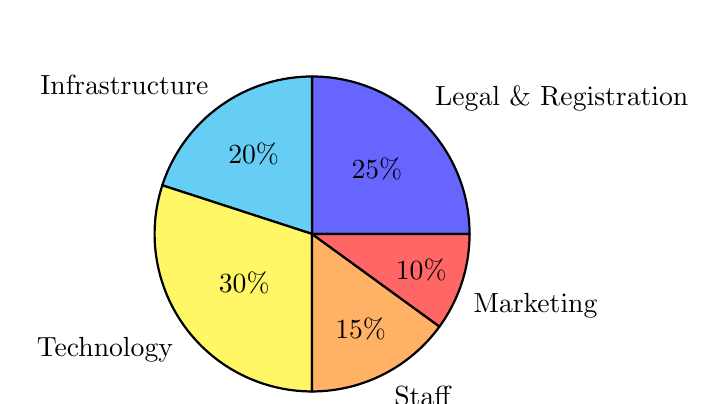
\begin{tikzpicture}
        % Pie chart for cost distribution
        \pie[radius=2]{
            25/Legal \& Registration,
            20/Infrastructure,
            30/Technology,
            15/Staff,
            10/Marketing
        }
    \end{tikzpicture}
    \caption{Typical Setup Cost Distribution}
\end{figure}

\subsection{Operating Expenses Framework}
\begin{tcolorbox}[colback=white,colframe=primarydark,title=\textbf{Monthly Operating Expenses}]
\begin{itemize}
    \item Staff Costs: \_\_\_\_\_\_\_\_\_
    \item Office/Infrastructure: \_\_\_\_\_\_\_\_\_
    \item Technology: \_\_\_\_\_\_\_\_\_
    \item Marketing: \_\_\_\_\_\_\_\_\_
    \item Professional Services: \_\_\_\_\_\_\_\_\_
    \item Contingency (15\%): \_\_\_\_\_\_\_\_\_
\end{itemize}
Total Monthly Burn Rate: \_\_\_\_\_\_\_\_\_
\end{tcolorbox}

\section{Revenue Projection Tools}

\subsection{Revenue Model Framework}
\begin{figure}[h]
    \centering
    \begin{tikzpicture}
        % Revenue projection graph
        \draw[->] (0,0) -- (10,0) node[right] {Time};
        \draw[->] (0,0) -- (0,6) node[above] {Revenue};
        \draw[blue, thick] (0,0) .. controls (3,2) and (6,4) .. (9,5);
        \draw[red, dashed] (0,0) .. controls (3,1) and (6,2) .. (9,3);
        \node[right] at (9,5) {Optimistic};
        \node[right] at (9,3) {Conservative};
    \end{tikzpicture}
    \caption{12-Month Revenue Projection Models}
\end{figure}

\section{Regional Financial Considerations}

\begin{regionalbox}{United Kingdom}
\textbf{Financial Services Investment Structure}
\begin{itemize}
    \item Regulatory capital requirements
    \item FCA compliance costs
    \item Cross-border transaction setup
    \item Professional indemnity insurance
\end{itemize}

\subsection{UK-Specific Costs}
\begin{center}
\begin{tabular}{p{0.4\textwidth}|p{0.5\textwidth}}
    \textbf{Cost Category} & \textbf{Typical Range (GBP)} \\
    \hline
    Regulatory Compliance & £20,000 - £50,000 \\
    Professional Services & £15,000 - £30,000 \\
    Technology Setup & £25,000 - £75,000 \\
\end{tabular}
\end{center}
\end{regionalbox}

\begin{regionalbox}{United States}
\textbf{Tech Startup Financial Framework}
\begin{itemize}
    \item Development team costs
    \item Infrastructure setup
    \item IP protection expenses
    \item Marketing budget
\end{itemize}

\subsection{US-Specific Costs}
\begin{center}
\begin{tabular}{p{0.4\textwidth}|p{0.5\textwidth}}
    \textbf{Cost Category} & \textbf{Typical Range (USD)} \\
    \hline
    Tech Development & \$50,000 - \$150,000 \\
    IP Protection & \$15,000 - \$30,000 \\
    Market Entry & \$25,000 - \$75,000 \\
\end{tabular}
\end{center}
\end{regionalbox}

\begin{regionalbox}{UAE}
\textbf{Trade Finance Options}
\begin{itemize}
    \item Trade license costs
    \item Warehouse setup
    \item Logistics infrastructure
    \item Working capital requirements
\end{itemize}

\subsection{UAE-Specific Costs}
\begin{center}
\begin{tabular}{p{0.4\textwidth}|p{0.5\textwidth}}
    \textbf{Cost Category} & \textbf{Typical Range (AED)} \\
    \hline
    Trade License & 50,000 - 100,000 \\
    Logistics Setup & 100,000 - 250,000 \\
    Working Capital & 200,000 - 500,000 \\
\end{tabular}
\end{center}
\end{regionalbox}

\begin{regionalbox}{Canada}
\textbf{Sector-Specific Grants and Support}
\begin{itemize}
    \item Government support programs
    \item Industry-specific grants
    \item R\&D tax credits
    \item Export development funding
\end{itemize}

\subsection{Canada-Specific Costs}
\begin{center}
\begin{tabular}{p{0.4\textwidth}|p{0.5\textwidth}}
    \textbf{Cost Category} & \textbf{Typical Range (CAD)} \\
    \hline
    Setup Costs & \$50,000 - \$150,000 \\
    Compliance & \$25,000 - \$75,000 \\
    Operations & \$100,000 - \$300,000 \\
\end{tabular}
\end{center}
\end{regionalbox}

\section{Funding Options and Sources}

\subsection{Funding Matrix}
\begin{center}
\begin{tabular}{p{0.2\textwidth}|p{0.2\textwidth}|p{0.2\textwidth}|p{0.3\textwidth}}
    \textbf{Source} & \textbf{Amount Range} & \textbf{Timeline} & \textbf{Requirements} \\
    \hline
    Self-Funding & Variable & Immediate & Personal assets \\
    Angel Investors & \$50k-\$250k & 1-3 months & Business plan \\
    Bank Finance & \$100k+ & 2-4 months & Collateral \\
    Grants & Variable & 3-6 months & Project proposal \\
\end{tabular}
\end{center}

\begin{communitybox}
Access additional financial planning resources on the Africa Growth Circle:
\begin{itemize}
    \item Financial modeling templates
    \item Investment readiness toolkit
    \item Funding source directory
    \item Expert financial advisory
\end{itemize}
Visit circle.counseal.com for financial planning support.
\end{communitybox}

% End of chapter workshop
\begin{workshopbox}
\textbf{Chapter 5 Financial Planning Workshop}

1. Investment Planning
\begin{itemize}
    \item Required startup capital: \_\_\_\_\_\_\_\_\_
    \item Funding sources identified: \_\_\_\_\_\_\_\_\_
    \item Timeline to funding: \_\_\_\_\_\_\_\_\_
\end{itemize}

2. Cost Structure
\begin{itemize}
    \item Setup costs breakdown: \_\_\_\_\_\_\_\_\_
    \item Monthly operating expenses: \_\_\_\_\_\_\_\_\_
    \item Contingency planning: \_\_\_\_\_\_\_\_\_
\end{itemize}

3. Revenue Projections
\begin{itemize}
    \item 6-month target: \_\_\_\_\_\_\_\_\_
    \item 12-month target: \_\_\_\_\_\_\_\_\_
    \item Key revenue drivers: \_\_\_\_\_\_\_\_\_
\end{itemize}

Download detailed financial planning templates from the Africa Growth Circle platform.
\end{workshopbox}

\begin{importantbox}
In Chapter 6, we'll explore risk management and compliance frameworks to protect your investment.
\end{importantbox}
    % chapters/06-risk-management.tex

\chapter{Risk Management and Compliance}\label{ch:risk-management-and-compliance}

\begin{importantbox}
This chapter provides a comprehensive framework for identifying, assessing, and mitigating risks in the Nigerian market, along with detailed compliance requirements by sector and region.
\end{importantbox}

\section{Due Diligence Framework}\label{sec:due-diligence-framework}

\subsection{Core Due Diligence Components}\label{subsec:core-due-diligence-components}

\begin{figure}[htbp]
    \centering
    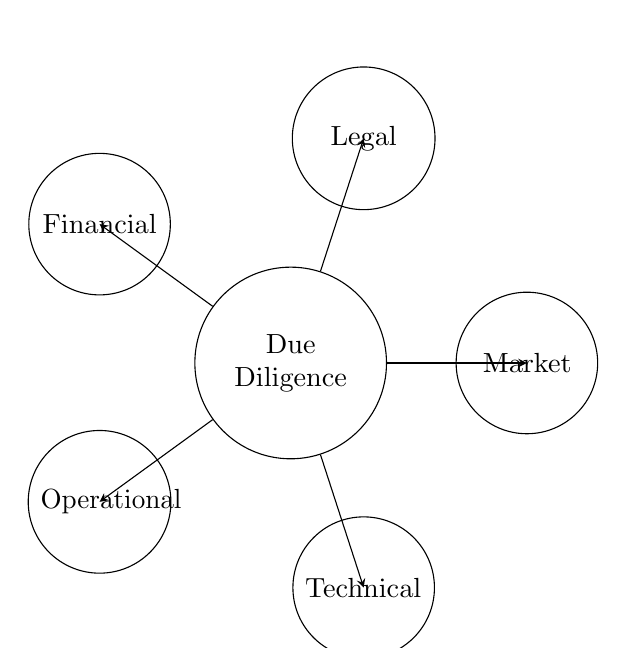
\begin{tikzpicture}[node distance=2cm]
        % Core node
        \node[draw, circle, text width=2cm, align=center] (core) {Due\\Diligence};

        % Surrounding nodes with better spacing
        \foreach \angle/\label in {
            0/Market,
            72/Legal,
            144/Financial,
            216/Operational,
            288/Technical
        } {
            \node[draw, circle, text width=1.5cm, align=center]
                at (\angle:3) {\label};
            \draw[-stealth] (core) -- (\angle:3);
        }
    \end{tikzpicture}
    \caption{Due Diligence Framework}
    \label{fig:due-diligence}
\end{figure}

\subsection{Risk Assessment Matrix}
\begin{center}
\begin{tabularx}{\textwidth}{>{\raggedright\arraybackslash}X >{\centering\arraybackslash}X >{\centering\arraybackslash}X >{\raggedright\arraybackslash}X}
    \toprule
    \textbf{Risk Type} & \textbf{Likelihood} & \textbf{Impact} & \textbf{Mitigation Strategy} \\
    \midrule
    Regulatory & High & High & Compliance partners \\
    Market & Medium & High & Phased entry \\
    Operational & Medium & Medium & Local expertise \\
    Financial & Medium & High & Risk management \\
    Technical & Low & Medium & Testing protocols \\
    \bottomrule
\end{tabularx}
\end{center}

\FloatBarrier
\section{Legal Safeguards}\label{sec:legal-safeguards}

\begin{warningbox}
Legal requirements can change frequently.\ Always verify current requirements through official channels or your legal counsel.
\end{warningbox}

\subsection{Essential Legal Documentation}\label{subsec:essential-legal-documentation}
\begin{tcolorbox}[colback=white,colframe=primarydark,title=\textbf{Documentation Checklist}]
\begin{itemize}
    \item Registration certificates
    \item Operating licenses
    \item Tax registrations
    \item Regulatory permits
    \item Employment contracts
    \item Partnership agreements
\end{itemize}
\end{tcolorbox}

\FloatBarrier
\section{Regional Compliance Requirements}\label{sec:regional-compliance-requirements}

\begin{regionalbox}{United Kingdom}
\textbf{Financial Services Compliance Framework}
\begin{itemize}
    \item \textbf{Central Bank of Nigeria (CBN) Requirements}
    \begin{itemize}
        \item Minimum capital requirement: NGN 25 billion for commercial banking
        \item Risk-based capital adequacy ratio: 15\%
        \item Non-performing loans ratio: maximum 5\%
        \item Liquidity ratio: minimum 30\%
        \item Daily reporting requirements for specified transactions
        \item Monthly returns submission
        \item Annual external audit
    \end{itemize}

    \item \textbf{Financial Conduct Authority (FCA) Requirements}
    \begin{itemize}
        \item Authorization application process
        \item Threshold Conditions compliance
        \item Systems and controls framework
        \item Senior Managers and Certification Regime
        \item Conduct risk management
        \item Client money protection
        \item Regular reporting obligations
    \end{itemize}

    \item \textbf{Anti-Money Laundering Regulations}
    \begin{itemize}
        \item Customer Due Diligence (CDD)
        \item Enhanced Due Diligence (EDD)
        \item Transaction monitoring systems
        \item Suspicious Activity Reporting (SAR)
        \item Record keeping requirements
        \item Staff training programs
        \item Regular risk assessments
    \end{itemize}

    \item \textbf{Data Protection Standards}
    \begin{itemize}
        \item Nigeria Data Protection Regulation compliance
        \item GDPR compliance for EU data
        \item Privacy impact assessments
        \item Data breach notification procedures
        \item Data retention policies
        \item Cross-border data transfer protocols
    \end{itemize}
\end{itemize}
\end{regionalbox}

\FloatBarrier
\subsection{UK Compliance Timeline}
\begin{figure}[htbp]
    \centering
    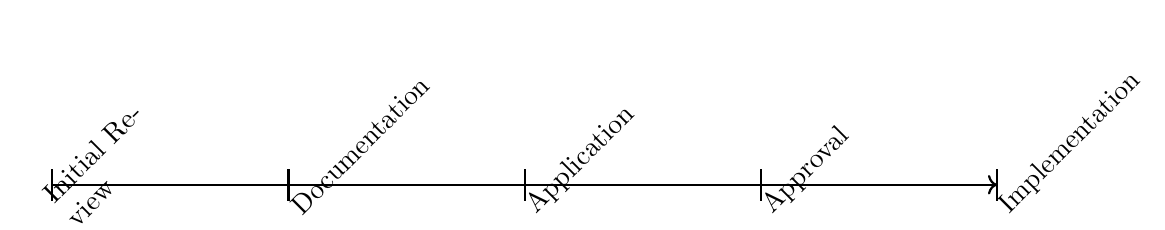
\begin{tikzpicture}
        % Timeline with better spacing and labels
        \draw[thick,->] (0,0) -- (12,0);
        \foreach \x/\label in {
            0/Initial Review,
            3/Documentation,
            6/Application,
            9/Approval,
            12/Implementation
        } {
            \draw[thick] (\x,0.2) -- (\x,-0.2);
            \node[text width=2cm, align=left, rotate=45, anchor=west]
                at (\x,-0.4) {\label};
        }
    \end{tikzpicture}
    \caption{UK Financial Services Compliance Process}
    \label{fig:uk-compliance}
\end{figure}

\begin{regionalbox}{United States}
\textbf{Tech Regulation and Data Protection}
\begin{itemize}
    \item \textbf{Data Privacy Requirements}
    \begin{itemize}
        \item NDPR compliance framework
        \item Privacy policy implementation
        \item Data collection consent
        \item Access rights management
        \item Breach notification protocols
        \item Regular privacy audits
    \end{itemize}

    \item \textbf{IP Protection Framework}
    \begin{itemize}
        \item Patent registration process
        \item Trademark protection
        \item Copyright registration
        \item Trade secret protocols
        \item Licensing agreements
        \item IP enforcement strategies
    \end{itemize}

    \item \textbf{Digital Security Compliance}
    \begin{itemize}
        \item Security assessment framework
        \item Penetration testing requirements
        \item Encryption standards
        \item Access control protocols
        \item Incident response planning
        \item Regular security audits
    \end{itemize}
\end{itemize}

\subsection{US Tech Compliance Matrix}\label{subsec:us-tech-compliance-matrix}
\begin{center}
\begin{tabularx}{\textwidth}{>{\raggedright\arraybackslash}X >{\centering\arraybackslash}X >{\raggedright\arraybackslash}X}
    \toprule
    \textbf{Requirement} & \textbf{Standard} & \textbf{Implementation} \\
    \midrule
    Data Privacy & NDPR/GDPR-aligned & Privacy framework \\
    Security & ISO 27001 & Security protocols \\
    Consumer Protection & FTC standards & Protection measures \\
    \bottomrule
\end{tabularx}
\end{center}
\end{regionalbox}

\begin{regionalbox}{UAE}
\textbf{Trade Compliance Framework}
\begin{itemize}
    \item \textbf{Trade License Requirements}
    \begin{itemize}
        \item General trading license
        \item Specific product licenses
        \item Agent registration
        \item Annual renewals
        \item Activity restrictions
    \end{itemize}

    \item \textbf{Import/Export Regulations}
    \begin{itemize}
        \item Documentation requirements
        \item Customs procedures
        \item Duty calculations
        \item Restricted items
        \item Special permissions
    \end{itemize}

    \item \textbf{Currency Controls}
    \begin{itemize}
        \item Transaction reporting
        \item Exchange controls
        \item Documentation requirements
        \item Transfer limits
        \item Compliance reporting
    \end{itemize}
\end{itemize}

\subsection{UAE Trade Compliance Checklist}\label{subsec:uae-trade-compliance-checklist}
\begin{tcolorbox}[colback=white,colframe=primary,title=\textbf{Required Documents}]
\begin{itemize}
    \item Trade license
    \item Chamber of Commerce registration
    \item Import/export permits
    \item Customs registration
    \item Bank references
\end{itemize}
\end{tcolorbox}
\end{regionalbox}

\begin{regionalbox}{Canada}
\textbf{Environmental and Agricultural Compliance}
\begin{itemize}
    \item Environmental standards
    \item Agricultural regulations
    \item Food safety requirements
    \item Export compliance
\end{itemize}

\subsection{Canadian Sector Compliance}\label{subsec:canadian-sector-compliance}
\begin{center}
\begin{tabularx}{\textwidth}{>{\raggedright\arraybackslash}X >{\centering\arraybackslash}X >{\raggedright\arraybackslash}X}
    \toprule
    \textbf{Sector} & \textbf{Standards} & \textbf{Certifications} \\
    \midrule
    Agriculture & CFIA standards & Safety certificates \\
    Environment & ISO 14001 & Environmental permits \\
    Food Processing & HACCP & Safety certifications \\
    \bottomrule
\end{tabularx}
\end{center}
\end{regionalbox}

\FloatBarrier
\section{Banking and Money Transfer}\label{sec:banking-and-money-transfer}

\subsection{Banking Structure}\label{subsec:banking-structure}
\begin{figure}[htbp]
    \centering
    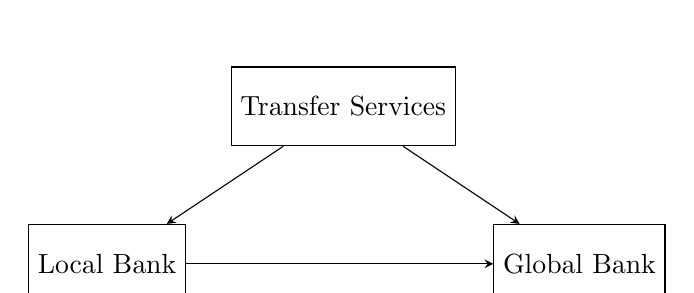
\begin{tikzpicture}[
        node distance=2cm,
        box/.style={draw, minimum width=2cm, minimum height=1cm}
    ]
        % Banking structure diagram with improved spacing
        \node[box] (local) at (0,0) {Local Bank};
        \node[box] (global) at (6,0) {Global Bank};
        \node[box] (transfer) at (3,2) {Transfer Services};
        \draw[-stealth] (local) -- (global);
        \draw[-stealth] (transfer) -- (local);
        \draw[-stealth] (transfer) -- (global);
    \end{tikzpicture}
    \caption{Cross-Border Banking Structure}
    \label{fig:banking-structure}
\end{figure}

\subsection{Banking Operations Framework}\label{subsec:banking-operations-framework}
\begin{tcolorbox}[colback=white,colframe=primarydark,title=\textbf{Banking Operations Components}]
\begin{itemize}
    \item \textbf{Account Setup}
    \begin{itemize}
        \item Corporate account requirements
        \item Documentation process
        \item Signatory arrangements
        \item Online banking setup
        \item Mobile banking activation
    \end{itemize}

    \item \textbf{Transaction Processing}
    \begin{itemize}
        \item Payment authorizations
        \item Transaction limits
        \item Processing timeframes
        \item Fee structures
        \item Reconciliation procedures
    \end{itemize}

    \item \textbf{Cross-Border Operations}
    \begin{itemize}
        \item International transfer protocols
        \item Documentation requirements
        \item Correspondent banking relationships
        \item Compliance procedures
        \item Reporting obligations
    \end{itemize}
\end{itemize}
\end{tcolorbox}

\FloatBarrier
\section{Currency Risk Management}\label{sec:currency-risk-management}

\subsection{Hedging Strategies Framework}\label{subsec:hedging-strategies-framework}
\begin{tcolorbox}[colback=white,colframe=primarydark,title=\textbf{Currency Risk Mitigation Strategies}]
\begin{itemize}
    \item \textbf{Forward Contracts}
    \begin{itemize}
        \item Contract specifications
        \item Pricing mechanisms
        \item Settlement procedures
        \item Documentation requirements
        \item Risk assessment
    \end{itemize}

    \item \textbf{Currency Hedging}
    \begin{itemize}
        \item Options strategies
        \item Swap arrangements
        \item Natural hedging
        \item Cross-currency hedging
        \item Cost considerations
    \end{itemize}

    \item \textbf{Local Currency Management}
    \begin{itemize}
        \item Account structuring
        \item Conversion timing
        \item Balance optimization
        \item Interest management
        \item Exposure limits
    \end{itemize}
\end{itemize}
\end{tcolorbox}

\begin{communitybox}
Access additional risk management resources on the Africa Growth Circle:
\begin{itemize}
    \item Risk assessment templates
    \item Compliance checklists
    \item Expert advisory sessions
    \item Regulatory updates
    \item Due diligence guides
\end{itemize}
Visit circle.counseal.com for risk management support.
\end{communitybox}

% End of chapter workshop
\begin{workshopbox}
\textbf{Chapter 6 Risk Management Workshop}

1. Risk Assessment
\begin{itemize}
    \item Key risks identified: \_\_\_\_\_\_\_\_\_
    \item Risk priority ranking: \_\_\_\_\_\_\_\_\_
    \item Mitigation strategies: \_\_\_\_\_\_\_\_\_
\end{itemize}

2. Compliance Planning
\begin{itemize}
    \item Required permits: \_\_\_\_\_\_\_\_\_
    \item Documentation needed: \_\_\_\_\_\_\_\_\_
    \item Timeline for completion: \_\_\_\_\_\_\_\_\_
\end{itemize}

3. Banking Structure
\begin{itemize}
    \item Banking partners: \_\_\_\_\_\_\_\_\_
    \item Transfer mechanisms: \_\_\_\_\_\_\_\_\_
    \item Currency management: \_\_\_\_\_\_\_\_\_
\end{itemize}

Download comprehensive risk assessment templates from the Africa Growth Circle platform.
\end{workshopbox}

\begin{importantbox}
In Chapter 7, we'll explore building your local network and establishing key partnerships to help manage risks and ensure compliance.
\end{importantbox}
    \chapter{Building Your Local Network}\label{ch:building-your-local-network}

I still remember the day Sarah called me in frustration.\ ``Dele,'' she sighed, ``I've been to three networking events this week, handed out countless business cards, but it feels like I'm getting nowhere.\ What am I missing?''

Her experience reminded me of my own early days building networks in Nigeria.\ Like many entrepreneurs, I initially approached networking with what I call the ``Silicon Valley mindset''—thinking relationships could be built through formal events and LinkedIn connections.\ It took me some time to understand that in Nigeria, real networks are built differently.

\section{Understanding Nigerian Business Networks}\label{sec:understanding-networks}

Let me share something I learned while building Firmbird: In Nigeria, business networks aren't just about professional connections --- they're about building trust circles.\ Think of it as joining a family rather than joining a LinkedIn group.

When I explained this to Sarah, her eyes lit up.\ ``That's why the quick connections weren't working,'' she realized.\ ``I was trying to rush relationships that need time to grow.''

Here's what I call the ``Trust Circle Principle'':

First Circle: Personal Connection
\begin{itemize}
    \item Start with genuine personal interest
    \item Share your story and listen to theirs
    \item Find common ground beyond business
    \item Build rapport before talking business
\end{itemize}

Second Circle: Professional Alignment
\begin{itemize}
    \item Identify mutual value opportunities
    \item Share industry insights and knowledge
    \item Offer help before asking for anything
    \item Build credibility through small actions
\end{itemize}

Third Circle: Business Integration
\begin{itemize}
    \item Start with small collaborations
    \item Prove reliability consistently
    \item Expand involvement gradually
    \item Maintain personal connections
\end{itemize}

\section{Regional Network Development}\label{sec:regional-networks}

Let me share what I've learned helping entrepreneurs from different regions build their Nigerian networks:

\subsection{European Approaches}\label{subsec:european-networks}

When Lisa, a founder from Manchester, first arrived in Lagos, she made what I call the ``Commonwealth Connection Mistake''—assuming shared history meant shared business culture.\ ``I thought our similar legal systems would make everything easier, '' she told me later, laughing. ``But I had to unlearn before I could learn.''

Here's what worked for her and other European entrepreneurs:

\begin{itemize}
    \item \textbf{Formal First, Personal Later}
    European entrepreneurs often succeed by starting with formal institutional connections (chambers of commerce, trade groups) but quickly learning to build personal relationships within these structures.

    \item \textbf{Documentation Balance}
    While maintaining European-style documentation, successful entrepreneurs learn to balance this with Nigerian relationship-based trust building.\ As one founder told me, ``The paperwork opens doors, but the relationships help you walk through them.''

    \item \textbf{Time Investment}
    European entrepreneurs who succeed typically plan for longer relationship-building periods than they're used to.\ ``In London, we might close a deal in one meeting, '' Lisa shared.\ ``Here, I learned to invest in five relationship-building meetings before even discussing business.''

    \item \textbf{Key Organizations}
    \begin{itemize}
        \item European Business Organization Nigeria
        \item European-Nigerian Chambers of Commerce
        \item EU-Nigeria Business Forum
        \item Regional Trade Missions
    \end{itemize}
\end{itemize}

\subsection{US/Canadian Networks}\label{subsec:north-american-networks}

North American entrepreneurs often bring what I call ``Speed Networking Syndrome''—expecting relationships to develop as quickly as they do in New York or Toronto.\ Here's how successful ones adapt:

\begin{itemize}
    \item \textbf{Community Integration}
    Rather than just focusing on business networks, successful North American entrepreneurs often engage with community initiatives first.\ This builds trust and opens doors naturally.

    \item \textbf{Patience Practice}
    ``I had to learn that a 15-minute coffee meeting wasn't going to cut it,'' one Boston entrepreneur told me.\ ``Now I plan for hour-long conversations that might not even touch on business.''

    \item \textbf{Value-First Approach}
    Successful North Americans learn to lead with value rather than opportunity.\ Share knowledge, make introductions, and build goodwill before discussing business potential.

    \item \textbf{Key Organizations}
    \begin{itemize}
        \item American Business Council
        \item US-Africa Business Center
        \item Canada-Nigeria Chamber of Commerce
        \item North American Trade Initiatives
    \end{itemize}
\end{itemize}

\subsection{UAE and Middle Eastern Approaches}\label{subsec:middle-eastern-networks}

Middle Eastern entrepreneurs often have a head start in understanding relationship-based business cultures, but Nigeria still requires specific adaptations:

\begin{itemize}
    \item \textbf{Cultural Bridge Building}
    Leverage understanding of relationship-based business while learning Nigerian-specific customs.\ As one Dubai-based entrepreneur told me, ``The principles are similar, but the practices are different.''

    \item \textbf{Long-term Vision}
    Build networks with multi-generational thinking.\ ``In Dubai, we think in decades,'' shared an Emirati founder.\ ``This mindset works well in Nigeria too.''

    \item \textbf{Trust Through Presence}
    Regular physical presence matters.\ Successful Middle Eastern entrepreneurs often maintain consistent visit schedules rather than trying to manage everything remotely.

    \item \textbf{Key Organizations}
    \begin{itemize}
        \item Nigerian-Arabian Gulf Chamber of Commerce
        \item Middle East Africa Trade Associations
        \item Islamic Chamber of Commerce
        \item Regional Business Councils
    \end{itemize}
\end{itemize}

\section{Practical Network Building}\label{sec:practical-networking}

Let me share what I call the ``Network Growth Framework'' --- a practical approach that's worked for entrepreneurs I've guided:

\subsection{First 30 Days}\label{subsec:first-30-days}

Start with what I call ``Foundation Connections'':
\begin{itemize}
    \item Join one relevant industry association
    \item Attend two industry-specific events
    \item Meet three potential mentors
    \item Connect with five peer entrepreneurs
\end{itemize}

\subsection{Days 31--60}\label{subsec:days-31-60}

Focus on ``Relationship Deepening'':
\begin{itemize}
    \item Follow up with key contacts personally
    \item Arrange one-on-one meetings
    \item Share valuable industry insights
    \item Offer help where possible
\end{itemize}

\subsection{Days 61--90}\label{subsec:days-61-90}

Begin ``Network Activation'':
\begin{itemize}
    \item Start small collaborations
    \item Introduce valuable connections
    \item Participate in industry initiatives
    \item Host small gatherings
\end{itemize}

\section{Digital Network Integration}\label{sec:digital-networks}

With internet penetration at 45.57\% and over 84\% of users accessing services via mobile, digital networking has become crucial.\ However, as I always tell entrepreneurs, ``Digital in Nigeria is a bridge, not a destination.''

Here's what works:
\begin{itemize}
    \item WhatsApp Business for daily communications
    \item LinkedIn for professional presence
    \item Industry-specific platforms for knowledge sharing
    \item Mobile-first communication strategies
\end{itemize}

\section{Workshop: Your Network Action Plan}\label{sec:network-workshop}

Let's turn these insights into action:

1. Network Mapping
\begin{itemize}
    \item List your top 5 network priorities: \_\_\_\_\_\_\_\_\_
    \item Identify 3 key industry associations: \_\_\_\_\_\_\_\_\_
    \item Map potential mentor connections: \_\_\_\_\_\_\_\_\_
\end{itemize}

2. Relationship Building
\begin{itemize}
    \item Weekly networking activities: \_\_\_\_\_\_\_\_\_
    \item Monthly relationship deepening: \_\_\_\_\_\_\_\_\_
    \item Quarterly network expansion: \_\_\_\_\_\_\_\_\_
\end{itemize}

3. Value Creation
\begin{itemize}
    \item What can you offer others?: \_\_\_\_\_\_\_\_\_
    \item Knowledge sharing plans: \_\_\_\_\_\_\_\_\_
    \item Collaboration opportunities: \_\_\_\_\_\_\_\_\_
\end{itemize}

Extra resources to support your networking journey are available at \href{https://viz.li/csl-book-ngbiz}{viz.li/csl-book-ngbiz}:
\begin{itemize}
    \item Network Tracking Template (Excel spreadsheet)
    \item Relationship Development Timeline (Interactive PDF)
    \item Industry Association Directory (Updated quarterly)
\end{itemize}

Remember what I told Sarah when she finally started seeing results: ``In Nigeria, we don't just build networks --- we build families.\ And family takes time, but it's worth every minute.''

In Chapter 8, we'll explore how to leverage these networks in setting up your operations effectively.
    % chapters/08-technology-operations.tex

\chapter{Technology and Operations}

\begin{importantbox}
This chapter provides comprehensive guidance on setting up your technology infrastructure and operations in Nigeria, with specific considerations for different business types and regions.
\end{importantbox}

\FloatBarrier
\section{Digital Infrastructure Setup}

\subsection{Core Technology Stack}
\begin{figure}[htbp]
    \centering
    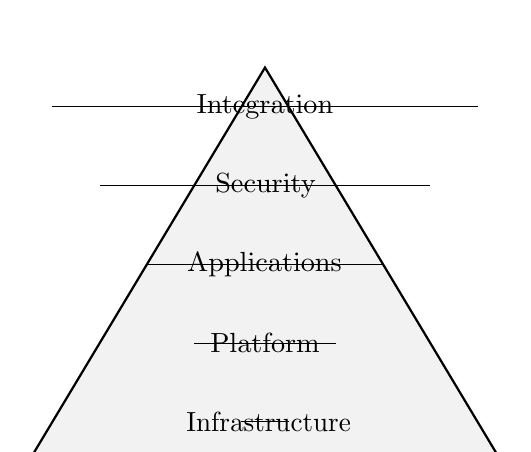
\begin{tikzpicture}[
        layer/.style={text width=2cm, align=center}
    ]
        % Technology stack pyramid with better proportions
        \fill[gray!10] (0,0) -- (6,0) -- (3,5) -- cycle;

        % Horizontal layers with better spacing
        \foreach \y/\label in {
            0.5/Infrastructure,
            1.5/Platform,
            2.5/Applications,
            3.5/Security,
            4.5/Integration
        } {
            \pgfmathsetmacro{\width}{6-\y*1.2}
            \draw (\width/2,\y) -- (6-\width/2,\y);
            \node[layer] at (3,\y) {\label};
        }

        % Outer pyramid
        \draw[thick] (0,0) -- (6,0) -- (3,5) -- cycle;
    \end{tikzpicture}
    \caption{Technology Stack Components}
    \label{fig:tech-stack}
\end{figure}

\subsection{Infrastructure Requirements Matrix}
\begin{center}
\begin{tabularx}{\textwidth}{>{\raggedright\arraybackslash}X >{\raggedright\arraybackslash}X >{\raggedright\arraybackslash}X >{\raggedright\arraybackslash}X}
    \toprule
    \textbf{Component} & \textbf{Basic} & \textbf{Advanced} & \textbf{Enterprise} \\
    \midrule
    Servers & Cloud-based & Hybrid & Multi-region \\
    Storage & Standard & Redundant & Distributed \\
    Network & Broadband & Dedicated & Multi-carrier \\
    Security & Essential & Enhanced & Comprehensive \\
    \bottomrule
\end{tabularx}
\end{center}

\section{Operations Management Framework}

\subsection{Core Operational Processes}
\begin{tcolorbox}[colback=white,colframe=primarydark,title=\textbf{Process Categories}]
\begin{itemize}
    \item Core Business Processes
    \item Support Functions
    \item Management Systems
    \item Quality Control
    \item Performance Monitoring
\end{itemize}
\end{tcolorbox}

\FloatBarrier
\section{Regional Technology Considerations}

% UK Region
\begin{regionalbox}{United Kingdom}
\textbf{Financial Services Systems}
\begin{itemize}
    \item Payment processing platforms
    \item Regulatory reporting systems
    \item Compliance monitoring tools
    \item Data protection infrastructure
\end{itemize}
\end{regionalbox}

\subsection{UK FinTech Architecture}
\begin{figure}[htbp]
    \centering
    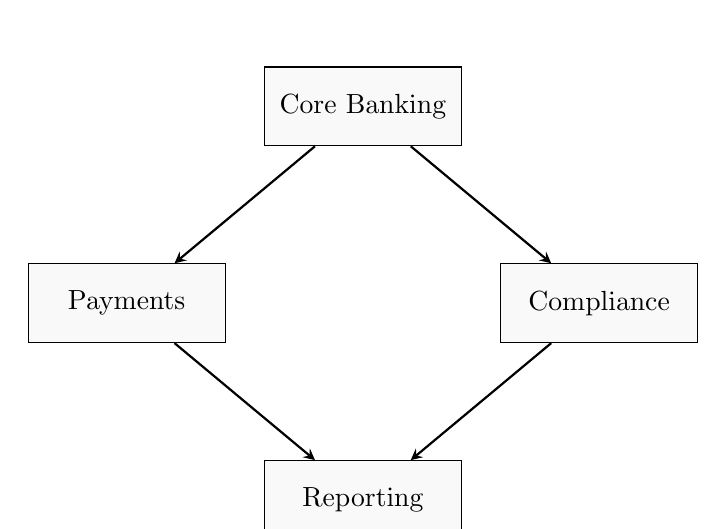
\begin{tikzpicture}[
        node distance=2.5cm,
        box/.style={draw, minimum width=2.5cm, minimum height=1cm, align=center, fill=gray!5},
        arrow/.style={-stealth, thick}
    ]
        % Financial systems architecture with improved layout
        \node[box] (core) at (0,0) {Core Banking};
        \node[box] (payment) at (-3,-2.5) {Payments};
        \node[box] (compliance) at (3,-2.5) {Compliance};
        \node[box] (reporting) at (0,-5) {Reporting};

        % Connect components with styled arrows
        \draw[arrow] (core) -- (payment);
        \draw[arrow] (core) -- (compliance);
        \draw[arrow] (payment) -- (reporting);
        \draw[arrow] (compliance) -- (reporting);
    \end{tikzpicture}
    \caption{Financial Services System Architecture}
    \label{fig:fintech-arch}
\end{figure}

% US Region
\begin{regionalbox}{United States}
\textbf{Tech Platform Integration}
\begin{itemize}
    \item Cloud infrastructure
    \item Development environments
    \item API integration
    \item Scalability framework
\end{itemize}
\end{regionalbox}

\subsection{US Tech Stack Implementation}
\begin{center}
\begin{tabularx}{\textwidth}{>{\raggedright\arraybackslash}X >{\raggedright\arraybackslash}X >{\raggedright\arraybackslash}X}
    \toprule
    \textbf{Layer} & \textbf{Components} & \textbf{Integration} \\
    \midrule
    Frontend & User Interface & API Gateway \\
    Backend & Business Logic & Microservices \\
    Database & Data Storage & Replication \\
    \bottomrule
\end{tabularx}
\end{center}

% UAE Region
\begin{regionalbox}{UAE}
\textbf{Trade and Logistics Systems}
\begin{itemize}
    \item Inventory management
    \item Supply chain tracking
    \item Customs documentation
    \item Logistics coordination
\end{itemize}

\subsection{UAE Trade Systems Architecture}
\begin{tcolorbox}[colback=white,colframe=primary,title=\textbf{System Components}]
\begin{enumerate}
    \item Order Management System
    \item Warehouse Management System
    \item Transportation Management System
    \item Documentation Management System
    \item Customs Interface
\end{enumerate}
\end{tcolorbox}
\end{regionalbox}

% Canada Region
\begin{regionalbox}{Canada}
\textbf{Industry-Specific Solutions}
\begin{itemize}
    \item Agricultural monitoring
    \item Environmental tracking
    \item Quality assurance systems
    \item Compliance monitoring
\end{itemize}

\subsection{Canadian Industry Solutions}
\begin{center}
\begin{tabularx}{\textwidth}{>{\raggedright\arraybackslash}X >{\raggedright\arraybackslash}X >{\raggedright\arraybackslash}X}
    \toprule
    \textbf{Industry} & \textbf{Core Systems} & \textbf{Integration Points} \\
    \midrule
    Agriculture & Field Management & Supply Chain \\
    Environment & Monitoring Tools & Reporting \\
    Manufacturing & Production Control & Quality Assurance \\
    \bottomrule
\end{tabularx}
\end{center}
\end{regionalbox}

\FloatBarrier
\section{Quality Control Systems}

\subsection{Quality Management Framework}
\begin{figure}[htbp]
    \centering
    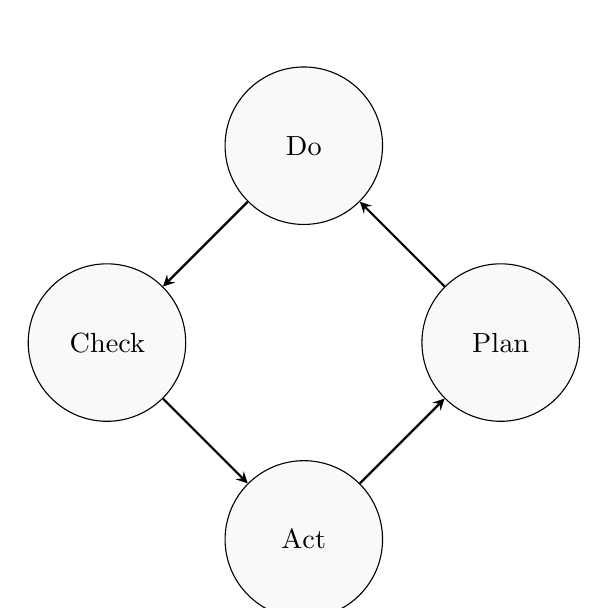
\begin{tikzpicture}[
        node distance=3cm,
        phase/.style={draw, circle, minimum size=2cm, text width=1.5cm, align=center, fill=gray!5},
        arrow/.style={-stealth, thick, bend left=15}
    ]
        % Quality management cycle with improved styling
        \foreach \angle/\label in {
            0/Plan,
            90/Do,
            180/Check,
            270/Act
        } {
            \node[phase] (phase-\angle) at (\angle:2.5) {\label};
        }

        % Connect phases with curved arrows
        \draw[arrow] (phase-0) -- (phase-90);
        \draw[arrow] (phase-90) -- (phase-180);
        \draw[arrow] (phase-180) -- (phase-270);
        \draw[arrow] (phase-270) -- (phase-0);
    \end{tikzpicture}
    \caption{Quality Management Cycle}
    \label{fig:quality-cycle}
\end{figure}

\section{Performance Monitoring}

\subsection{KPI Dashboard Framework}
\begin{tcolorbox}[colback=white,colframe=primarydark,title=\textbf{Key Performance Indicators}]
\begin{itemize}
    \item Operational Efficiency
    \item System Uptime
    \item Process Compliance
    \item Error Rates
    \item Response Times
\end{itemize}
\end{tcolorbox}

\begin{communitybox}
Access technology and operations resources on the Africa Growth Circle:
\begin{itemize}
    \item System setup guides
    \item Vendor recommendations
    \item Implementation templates
    \item Tech support network
    \item Operations best practices
\end{itemize}
Visit circle.counseal.com for technology support.
\end{communitybox}

\begin{workshopbox}
\textbf{Chapter 8 Technology Planning Workshop}

1. Infrastructure Planning
\begin{itemize}
    \item Core systems needed: \_\_\_\_\_\_\_\_\_
    \item Integration requirements: \_\_\_\_\_\_\_\_\_
    \item Security considerations: \_\_\_\_\_\_\_\_\_
\end{itemize}

2. Operations Setup
\begin{itemize}
    \item Process documentation: \_\_\_\_\_\_\_\_\_
    \item Quality controls: \_\_\_\_\_\_\_\_\_
    \item Performance metrics: \_\_\_\_\_\_\_\_\_
\end{itemize}

3. Implementation Timeline
\begin{itemize}
    \item System selection: \_\_\_\_\_\_\_\_\_
    \item Setup phases: \_\_\_\_\_\_\_\_\_
    \item Testing schedule: \_\_\_\_\_\_\_\_\_
\end{itemize}

Download technical implementation guides from the Africa Growth Circle platform.
\end{workshopbox}

\begin{importantbox}
In Chapter 9, we'll explore strategies for growth and scaling your operations once your technology infrastructure is in place.
\end{importantbox}
    \chapter{Growth and Scaling Strategies}\label{ch:growth-and-scaling-strategies}

I remember Sarah, the fintech founder we met earlier.\ She had successfully launched her payment solution, gaining steady traction in her initial market segment.\ ``Dele,'' she said, stirring her drink thoughtfully, ``we've got the foundation right.\ But how do we really scale this thing?''

That question --- how to scale effectively in Nigeria --- is one I've heard countless times, in different accents, from entrepreneurs across various sectors.\ The answer, I've learned, isn't just about having the right strategy on paper.\ It's about understanding what I call the ``Nigerian Scale Dance'' --- the delicate balance between ambition and reality, between speed and sustainability.

\begin{importantbox}
    When Sarah returned much later, her business had increased in size --- not because she followed some generic growth playbook, but because she'd learned to dance to Nigeria's unique rhythm.\ This chapter will show you how to master that same dance.
\end{importantbox}


\section{The Scale-Smart Framework}\label{sec:scale-smart-framework}

Let me share something I learned while scaling Firmbird: In Nigeria, scaling isn't just about getting bigger --- it's about getting smarter.\ Here's what I call the ``Scale-Smart Matrix'':

\begin{tcolorbox}[colback=white,colframe=primarydark,title=\textbf{Scale-Smart Components}]
    \begin{itemize}
        \item \textbf{Systems}
        Build processes that can handle 10x your current volume

        \item \textbf{Market}
        Understand which segments are ready for expansion

        \item \textbf{Assets}
        Invest in scalable resources and relationships

        \item \textbf{Risk}
        Maintain control as you accelerate growth

        \item \textbf{Team}
        Develop leadership that can drive sustainable expansion
    \end{itemize}
\end{tcolorbox}

Remember Mike, our e-commerce entrepreneur from Chapter 3? His first attempt at scaling nearly broke his business.\ ``I thought scaling meant doing everything bigger, '' he told me later.\ ``I learned it actually means doing everything better.''


\section{Implementation Framework}\label{sec:future-ready-implementation-framework}

``Theory without implementation is just wishful thinking,'' I told Sarah.\ Here's the practical framework I call the ``Future-Ready Implementation Matrix'':

\begin{tcolorbox}[colback=white,colframe=primarydark,title=\textbf{Digital Acceleration: Implementation Steps}]
    \begin{enumerate}
        \item \textbf{Infrastructure Assessment}
        \begin{itemize}
            \item Create digital asset inventory spreadsheet
            \item Rate each system's scalability (1-5 scale)
            \item Document failure points and bottlenecks
            \item Calculate cost per transaction/interaction
            \item Set monthly review cycles
        \end{itemize}

        \item \textbf{Customer Journey Mapping}
        \begin{itemize}
            \item Create detailed interaction flowcharts
            \item Identify manual processes for automation
            \item List all customer friction points
            \item Prioritize improvements (Impact vs.\ Effort matrix)
            \item Set quarterly review cycles
        \end{itemize}

        \item \textbf{Phased Implementation}
        \begin{itemize}
            \item Select pilot department/process
            \item Run parallel systems during transition
            \item Document daily learning points
            \item Train staff in structured batches
            \item Monitor KPIs weekly
        \end{itemize}
    \end{enumerate}
\end{tcolorbox}

\begin{tcolorbox}[colback=white,colframe=primarydark,title=\textbf{Economic Rebalancing: Action Steps}]
    \begin{enumerate}
        \item \textbf{Financial Planning}
        \begin{itemize}
            \item Create 13-week rolling cash flow forecast
            \item Map revenue-expense currency matching
            \item Build 3-month expense buffer
            \item Set monthly review cycles
        \end{itemize}

        \item \textbf{Risk Management}
        \begin{itemize}
            \item Develop currency hedging strategy
            \item Create supplier diversification plan
            \item Build pricing flexibility mechanisms
            \item Set bi-weekly review cycles
        \end{itemize}

        \item \textbf{Growth Planning}
        \begin{itemize}
            \item Map sector growth opportunities
            \item Create resource allocation matrix
            \item Build capacity expansion timeline
            \item Set quarterly review cycles
        \end{itemize}
    \end{enumerate}
\end{tcolorbox}


\section{Technology Evolution Framework}\label{sec:tech-evolution-framework}

When Mike asked about technology preparation, I shared what I call the ``Tech Evolution Pyramid'':

\begin{tcolorbox}[colback=white,colframe=primarydark,title=\textbf{Technology Implementation Steps}]
    \begin{enumerate}
        \item \textbf{Infrastructure Modernization}
        \begin{itemize}
            \item Audit current technology stack
            \item Identify cloud migration opportunities
            \item Plan edge computing implementation
            \item Create backup system protocols
            \item Set weekly monitoring cycles
        \end{itemize}

        \item \textbf{Security Enhancement}
        \begin{itemize}
            \item Implement multi-layer security
            \item Create incident response plans
            \item Deploy automated monitoring
            \item Conduct regular penetration testing
            \item Set daily review cycles
        \end{itemize}

        \item \textbf{Integration Development}
        \begin{itemize}
            \item Map all system interconnections
            \item Create API documentation
            \item Build microservices architecture
            \item Implement real-time monitoring
            \item Set monthly review cycles
        \end{itemize}
    \end{enumerate}
\end{tcolorbox}


\section{Workforce Evolution}\label{sec:workforce-development}

Lisa's AgriTech success taught us the importance of what I call the ``People Development Pipeline'':

\begin{tcolorbox}[colback=white,colframe=primarydark,title=\textbf{Workforce Development Steps}]
    \begin{enumerate}
        \item \textbf{Skills Assessment}
        \begin{itemize}
            \item Create skills matrix for each role
            \item Map current vs.\ future skills gaps
            \item Develop individual learning paths
            \item Build internal training programs
            \item Set quarterly assessments
        \end{itemize}

        \item \textbf{Culture Building}
        \begin{itemize}
            \item Define core values and behaviors
            \item Create innovation reward systems
            \item Implement feedback mechanisms
            \item Build cross-functional teams
            \item Set monthly culture checks
        \end{itemize}

        \item \textbf{Knowledge Management}
        \begin{itemize}
            \item Create central knowledge repository
            \item Implement mentorship programs
            \item Build skill-sharing platforms
            \item Document best practices
            \item Set weekly knowledge shares
        \end{itemize}
    \end{enumerate}
\end{tcolorbox}


\section{Market Positioning Strategy}\label{sec:market-positioning-strategy}

Ahmed's success in adapting his trading business showed us the power of what I call the ``Market Evolution Matrix'':

\begin{tcolorbox}[colback=white,colframe=primarydark,title=\textbf{Market Positioning Steps}]
    \begin{enumerate}
        \item \textbf{Market Analysis}
        \begin{itemize}
            \item Create competitor tracking system
            \item Map customer segment evolution
            \item Monitor regulatory changes
            \item Track technology trends
            \item Set monthly market reviews
        \end{itemize}

        \item \textbf{Product Evolution}
        \begin{itemize}
            \item Build product development pipeline
            \item Create feature prioritization system
            \item Implement A/B testing framework
            \item Monitor user feedback
            \item Set bi-weekly product reviews
        \end{itemize}

        \item \textbf{Customer Engagement}
        \begin{itemize}
            \item Develop omnichannel strategy
            \item Create customer feedback loops
            \item Build loyalty programs
            \item Monitor satisfaction metrics
            \item Set daily engagement reviews
        \end{itemize}
    \end{enumerate}
\end{tcolorbox}


\section{Risk Management Framework}\label{sec:risk-management-framework}

Looking ahead to 2025 and beyond, I advised Sarah to implement what I call the ``Resilience Framework'':

\begin{tcolorbox}[colback=white,colframe=primarydark,title=\textbf{Risk Management Implementation}]
    \begin{enumerate}
        \item \textbf{Risk Identification}
        \begin{itemize}
            \item Create risk assessment checklist
            \item Assign risk owners by area
            \item Track incidents and near-misses
            \item Monitor external threats
            \item Set weekly risk reviews
        \end{itemize}

        \item \textbf{Mitigation Planning}
        \begin{itemize}
            \item Build response playbooks
            \item Create emergency procedures
            \item Test backup systems
            \item Document lessons learned
            \item Set monthly mitigation reviews
        \end{itemize}

        \item \textbf{Control Implementation}
        \begin{itemize}
            \item Deploy monitoring systems
            \item Create reporting frameworks
            \item Build escalation procedures
            \item Test response scenarios
            \item Set daily control checks
        \end{itemize}
    \end{enumerate}
\end{tcolorbox}

\section{Action Planning Workshop}\label{sec:action-planning-workshop-9}

\begin{workshopbox}
    \textbf{Future-Proofing Action Plan}

    1. Technology Assessment
    \begin{itemize}
        \item Current capabilities: \_\_\_\_\_\_\_\_\_
        \item Required upgrades: \_\_\_\_\_\_\_\_\_
        \item Implementation timeline: \_\_\_\_\_\_\_\_\_
    \end{itemize}

    2. Market Position
    \begin{itemize}
        \item Competitive advantages: \_\_\_\_\_\_\_\_\_
        \item Growth opportunities: \_\_\_\_\_\_\_\_\_
        \item Resource requirements: \_\_\_\_\_\_\_\_\_
    \end{itemize}

    3. Risk Management
    \begin{itemize}
        \item Key risks identified: \_\_\_\_\_\_\_\_\_
        \item Mitigation strategies: \_\_\_\_\_\_\_\_\_
        \item Monitoring mechanisms: \_\_\_\_\_\_\_\_\_
    \end{itemize}
\end{workshopbox}

\begin{communitybox}
    Access additional resources on the Africa Growth Circle:
    \begin{itemize}
        \item Economic forecasting tools
        \item Risk assessment frameworks
        \item Expert advisory sessions
        \item Implementation templates
    \end{itemize}
    Visit \href{https://viz.li/csl-book-ngbiz}{viz.li/csl-book-ngbiz} for ongoing support.
\end{communitybox}

\begin{importantbox}
    As Sarah concluded, she had a clear roadmap for the years ahead.\ ``It's not about predicting every change, '' she reflected, ``but building a business that can adapt to any change.''

    Remember, in Nigeria's evolving landscape, the most successful businesses won't just react to change—they'll help shape it.\ The future belongs to those who prepare for it today.
\end{importantbox}

    \chapter{Future-Proofing Your Business}\label{ch:future-proofing-your-business}

I was sitting with Sarah in her Lagos office, now significantly expanded from when we first met. The screens behind her displayed real-time transaction data from her fintech platform. ``Dele,'' she said, pointing to a graph showing rising digital payment volumes, ``we're seeing incredible growth, but I keep thinking about what's next. How do we make sure we're building for 2025, not just 2024?''

Her question strikes at the heart of what every forward-thinking entrepreneur in Nigeria needs to consider. The answer lies not just in predicting the future, but in building businesses resilient enough to thrive in any future.

\section{Understanding Tomorrow's Market}\label{sec:understanding-tomorrow}

Let me share something I learned while helping businesses navigate Nigeria's evolving landscape: The most successful companies don't just adapt to change --- they position themselves to benefit from it. Here's what I call the ``Triple Wave'' that will shape Nigeria's business environment through 2025:

\subsection{Digital Transformation}\label{subsec:digital-transformation}

When a Canadian tech founder asked me about Nigeria's digital readiness, I showed him three numbers that changed his perspective:
\begin{itemize}
    \item 45.57\% internet penetration and growing
    \item 84\% of users accessing services via mobile
    \item 71.46\% tele-density with 154.9m active subscribers
\end{itemize}

``But what do these numbers mean for my business?'' he asked. Here's what I told him: ``They mean your digital strategy isn't just about having a website --- it's about building a business that lives in your customers' phones.''

\subsection{Economic Evolution}\label{subsec:economic-evolution}

The projections paint an interesting picture:
\begin{itemize}
    \item GDP growth reaching 4.12\% by 2025
    \item MPR moderating to 22.25\%
    \item Inflation trending toward 21.60\%
\end{itemize}

But these aren't just numbers. As I told Sarah, ``These trends are your business opportunities if you know how to read them.''

\subsection{Consumer Revolution}\label{subsec:consumer-revolution}

Nigeria's consumer landscape is transforming in three critical ways:
\begin{itemize}
    \item Rising urbanization (54.28\% and growing)
    \item Youthful population (median age 19.2 years)
    \item Expanding middle class through consumer credit reforms
\end{itemize}

\section{Building Your Future-Ready Framework}\label{sec:future-ready-framework}

When Mike asked me about preparing his e-commerce platform for 2025, I shared what I call the ``Future-Ready Matrix.'' Here's how to implement it:

\subsection{Technology Foundation}\label{subsec:tech-foundation}

Start with what I call the ``2025 Tech Stack'':

\begin{itemize}
    \item \textbf{Core Infrastructure}
    \begin{itemize}
        \item Cloud-based operations (\$150-300/month)
        \item Mobile-first architecture
        \item API-driven integrations
        \item Automated backup systems
    \end{itemize}

    \item \textbf{Security Framework}
    \begin{itemize}
        \item Multi-factor authentication
        \item Encrypted data storage
        \item Regular security audits
        \item Incident response protocols
    \end{itemize}

    \item \textbf{Scalability Features}
    \begin{itemize}
        \item Load balancing capabilities
        \item Microservices architecture
        \item Container deployment
        \item Performance monitoring
    \end{itemize}
\end{itemize}

\subsection{CALM Fund Integration}\label{subsec:calm-integration}

Sarah's success with the CALM Fund offers valuable lessons. Here's how she structured her future-ready investment:

\begin{itemize}
    \item \textbf{Power Infrastructure}
    \begin{itemize}
        \item Solar system financing (24\% annual interest)
        \item 2-year payment plan (\$150 monthly)
        \item 60\% reduction in power costs
        \item Backup power guarantee
    \end{itemize}

    \item \textbf{Mobility Solutions}
    \begin{itemize}
        \item CNG vehicle conversion
        \item Reduced operational costs
        \item Environmental compliance
        \item Future-proof transportation
    \end{itemize}
\end{itemize}

\subsection{SCALE Program Implementation}\label{subsec:scale-implementation}

Mike's e-commerce platform leveraged SCALE for future growth:

\begin{itemize}
    \item \textbf{Digital Infrastructure}
    \begin{itemize}
        \item Equipment financing
        \item Technology package deals
        \item Flexible payment terms
        \item Scalable solutions
    \end{itemize}

    \item \textbf{Customer Solutions}
    \begin{itemize}
        \item Consumer financing integration
        \item Reduced payment defaults
        \item Increased order values
        \item Customer loyalty programs
    \end{itemize}
\end{itemize}

\section{Workforce Evolution}\label{sec:workforce-evolution}

Lisa's AgriTech success taught us valuable lessons about future-ready teams:

\subsection{Skill Development}\label{subsec:skill-development}
\begin{itemize}
    \item Digital competency training
    \item Leadership development
    \item Cross-functional capabilities
    \item Innovation mindset building
\end{itemize}

\subsection{Culture Building}\label{subsec:culture-building}
\begin{itemize}
    \item Remote work protocols
    \item Digital collaboration tools
    \item Performance measurement
    \item Knowledge sharing systems
\end{itemize}

\section{Risk Management 2025}\label{sec:risk-2025}

I helped Sarah implement what I call the ``Future Risk Framework'':

\begin{itemize}
    \item \textbf{Technology Risks}
    \begin{itemize}
        \item Cybersecurity protocols
        \item Data protection measures
        \item System redundancy
        \item Recovery procedures
    \end{itemize}

    \item \textbf{Market Risks}
    \begin{itemize}
        \item Competitor monitoring
        \item Consumer trend tracking
        \item Regulatory compliance
        \item Economic impact assessment
    \end{itemize}

    \item \textbf{Operational Risks}
    \begin{itemize}
        \item Supply chain resilience
        \item Quality control systems
        \item Process automation
        \item Performance monitoring
    \end{itemize}
\end{itemize}

\section{Implementation Workshop}\label{sec:implementation-workshop-main}

Let's turn these insights into action:

\begin{enumerate}
    \item \textbf{Technology Assessment}
    \begin{itemize}
        \item Map current capabilities
        \item Identify future needs
        \item Plan upgrade path
        \item Budget allocation
    \end{itemize}

    \item \textbf{Market Position}
    \begin{itemize}
        \item Competitive analysis
        \item Growth opportunities
        \item Resource requirements
        \item Implementation timeline
    \end{itemize}

    \item \textbf{Risk Management}
    \begin{itemize}
        \item Risk identification
        \item Mitigation strategies
        \item Monitoring systems
        \item Response protocols
    \end{itemize}
\end{enumerate}

To support your future-proofing journey, I've created several practical tools available at viz.li/csl-book-ngbiz:

\begin{itemize}
    \item \textbf{Future-Proofing Calculator}
    An Excel-based tool for modeling growth scenarios and investments

    \item \textbf{Technology Stack Planner}
    Interactive worksheet for mapping infrastructure needs

    \item \textbf{Risk Assessment Matrix}
    Customizable template with Nigerian market-specific factors

    \item \textbf{Implementation Timeline Generator}
    Visual project management tool for transformation planning
\end{itemize}

Remember what I told Sarah when she worried about getting everything perfect: ``The future isn't about predicting every change --- it's about building a business that can adapt to any change.''

As you implement these strategies, remember that success in Nigeria's evolving landscape doesn't come from having the most sophisticated plans, but from having the most adaptable ones. The entrepreneurs who will thrive in 2025 and beyond are those building resilient, adaptable businesses today.

\begin{importantbox}
With projected GDP growth of 4.12\% in 2025 and significant reforms underway, Nigeria's business landscape is evolving rapidly. Your success will depend not on predicting every change, but on building a business that can adapt to and thrive in any future scenario.
\end{importantbox}

\begin{workshopbox}
\textbf{Future-Proofing Action Plan}

1. Technology Readiness
\begin{itemize}
    \item Current capabilities: \_\_\_\_\_\_\_\_\_
    \item Required upgrades: \_\_\_\_\_\_\_\_\_
    \item Implementation timeline: \_\_\_\_\_\_\_\_\_
\end{itemize}

2. Market Evolution
\begin{itemize}
    \item Growth opportunities: \_\_\_\_\_\_\_\_\_
    \item Required resources: \_\_\_\_\_\_\_\_\_
    \item Action steps: \_\_\_\_\_\_\_\_\_
\end{itemize}

3. Risk Preparation
\begin{itemize}
    \item Key risks: \_\_\_\_\_\_\_\_\_
    \item Mitigation strategies: \_\_\_\_\_\_\_\_\_
    \item Monitoring plan: \_\_\_\_\_\_\_\_\_
\end{itemize}
\end{workshopbox}

\begin{communitybox}
Access additional future-proofing resources at viz.li/csl-book-ngbiz:
\begin{itemize}
    \item Future-Proofing Strategy Templates
    \item Technology Investment Calculator
    \item Risk Assessment Tools
    \item Implementation Guides
\end{itemize}
Each tool includes step-by-step instructions and can be customized for your specific business needs.
\end{communitybox}

\section{Conclusion: Your Nigerian Journey}\label{sec:conclusion}

As we conclude this journey together, let me share something I told Sarah recently as we reflected on her progress from that first nervous meeting to her current success: ``The real opportunity in Nigeria isn't just in the market size or growth numbers --- it's in the chance to build something truly meaningful.''

Throughout this book, we've explored:

\begin{itemize}
    \item \textbf{Understanding the Real Nigeria} (Chapter 1)
    Moving beyond headlines to grasp the true dynamics of Africa's largest market

    \item \textbf{Strategic Entry} (Chapters 2-4)
    Building a solid foundation through careful planning, strong relationships, and strategic positioning

    \item \textbf{Operational Excellence} (Chapters 5-8)
    Mastering the practical aspects of finance, risk management, networking, and technology

    \item \textbf{Sustainable Growth} (Chapters 9-10)
    Creating resilient businesses ready for both today's challenges and tomorrow's opportunities
\end{itemize}

But more importantly, we've seen these principles come to life through the stories of entrepreneurs like Sarah, Mike, Lisa, and Ahmed --- real people who transformed their Nigerian business dreams into reality.

The economic indicators paint an encouraging picture: 4.12\% GDP growth projected for 2025, urbanization exceeding 54\%, internet penetration at 45.57\%, and significant reforms reshaping the financial landscape. But as I always tell entrepreneurs, these numbers aren't just statistics --- they're opportunities waiting for the right vision and execution.

Your next steps should be:

\begin{enumerate}
    \item Review your Market Entry Readiness Assessment from Chapter 1
    \item Download and complete the implementation tools from viz.li/csl-book-ngbiz
    \item Begin building your local network using the frameworks from Chapter 7
    \item Create your 90-day action plan following Chapter 4's guidelines
\end{enumerate}

Remember the Yoruba proverb I shared earlier: ``Ọ̀nà kan ò wọ ọjà'' --- there isn't just one path to the market. Your journey in Nigeria will be uniquely yours, but you don't have to walk it alone. The principles, tools, and insights in this book, combined with the resources at viz.li/csl-book-ngbiz, are here to guide your steps.

As you move forward, remember what that UK entrepreneur told me after successfully launching his business: ``Nigeria didn't just give me a market --- it gave me a new way of seeing business opportunities everywhere.''

Your Nigerian journey starts now. Make it count.

As I've shared throughout this book, successful market entry isn't just about having the right information --- it's about having the right support. If you'd like to continue this conversation or need guidance on your Nigerian market journey, you can reach me and my team through:

\begin{itemize}
    \item Website: \href{https://counseal.com}{counseal.com}
    \item Phone/WhatsApp: \href{https://wa.me/2348123307731}{+234 812 330 7731}
    \item Email: \href{mailto:ask@counseal.com?subject=Question%20from%20Book}{ask@counseal.com}
    \item Twitter: \href{https://twitter.com/getcounseal}{@getcounseal}
\end{itemize}

Whether you're ready to start your Nigerian market entry journey or just exploring possibilities, our team is here to help turn your business vision into reality. Check counseal.com for the latest market insights, success stories, and implementation support.

Remember, your success in Nigeria is not just about what you know, but who you know. Let's make your Nigerian business dreams a reality.

\begin{flushright}
\textit{-- Dele Omotosho\\
Lagos, Nigeria\\
February 2025}
\end{flushright}

    \backmatter

    % appendix/templates.tex

\chapter{Document Templates by Region}

\begin{importantbox}
This appendix provides essential document templates for business setup and operations. Additional templates and updates are available on the Africa Growth Circle platform.
\end{importantbox}

\section{United Kingdom Templates}
\begin{tcolorbox}[colback=white,colframe=primarydark,title=\textbf{Financial Services Documentation}]
\begin{itemize}
    \item Regulatory compliance checklist
    \item FCA application framework
    \item Risk assessment template
    \item Due diligence questionnaire
    \item Partnership agreement template
\end{itemize}
\end{tcolorbox}

\section{United States Templates}
\begin{tcolorbox}[colback=white,colframe=primarydark,title=\textbf{Tech Business Documentation}]
\begin{itemize}
    \item IP protection filing template
    \item Tech partnership agreement
    \item Service level agreement
    \item Data protection policy
    \item User agreement template
\end{itemize}
\end{tcolorbox}
    % appendix/checklists.tex

\chapter{Regulatory Compliance Checklists}

\begin{importantbox}
    These checklists provide structured guidance for meeting regulatory requirements. Updated versions are maintained on the Africa Growth Circle platform.
\end{importantbox}


\section{Business Registration}
\begin{center}
    \begin{tabular}{p{0.4\textwidth}|p{0.2\textwidth}|p{0.3\textwidth}}
        \textbf{Requirement}       & \textbf{Timeline} & \textbf{Authority} \\
        \hline
        Business Name Registration & 1-2 weeks         & CAC                \\
        Tax Registration           & 1 week            & FIRS               \\
        Industry License           & 2-4 weeks         & Varies             \\
    \end{tabular}
\end{center}
    % appendix/directory.tex

\chapter{Service Provider Directory}

\begin{importantbox}
    This directory provides a curated list of verified service providers. The complete, regularly updated directory is available on the Africa Growth Circle platform.
\end{importantbox}


\section{Legal Services}
\begin{tcolorbox}[colback=white,colframe=primarydark,title=\textbf{Legal Service Categories}]
    \begin{itemize}
        \item Corporate Law
        \item Regulatory Compliance
        \item Intellectual Property
        \item Employment Law
        \item Contract Law
    \end{itemize}
\end{tcolorbox}
    % appendix/resources.tex

\chapter{Regional Resource Guide}\label{ch:regional-resources}

\begin{importantbox}
    This guide provides key resources and contacts by region. Additional resources and regular updates are available on the Africa Growth Circle platform.
\end{importantbox}


\section{Government Agencies}\label{sec:government-agencies}
\vspace{1em}

\begin{center}
    \begin{tabularx}{\textwidth}{>{\raggedright\arraybackslash}X >{\raggedright\arraybackslash}X >{\raggedright\arraybackslash}X}
        \toprule
        \textbf{Agency}                         & \textbf{Role}           & \textbf{Contact} \\
        \midrule
        Corporate Affairs Commission            & Business Registration   & www.cac.gov.ng   \\
        Federal Inland Revenue Service          & Tax Administration      & www.firs.gov.ng  \\
        Central Bank of Nigeria                 & Banking Regulation      & www.cbn.gov.ng   \\
        Nigeria Investment Promotion Commission & Investment Facilitation & www.nipc.gov.ng  \\
        Standards Organization of Nigeria       & Quality Standards       & www.son.gov.ng   \\
        \bottomrule
    \end{tabularx}
\end{center}


\section{Regional Business Support Centers}\label{sec:support-centers}
\vspace{1em}

\begin{tcolorbox}[
    colback=white,
    colframe=primarydark,
    title=\textbf{Lagos Region},
    before skip=1em,
    after skip=1em
]
    \begin{itemize}[leftmargin=*,itemsep=0.5em]
        \item \textbf{Business Registration Support}
        \begin{itemize}[itemsep=0.3em]
            \item CAC Lagos Office
            \item Business Registration Support Desk
            \item Document Processing Center
            \item Verification Services
        \end{itemize}

        \vspace{0.5em}

        \item \textbf{Tax Support Services}
        \begin{itemize}[itemsep=0.3em]
            \item FIRS Tax Office
            \item Tax Consultation Center
            \item Documentation Support
            \item Advisory Services
        \end{itemize}

        \vspace{0.5em}

        \item \textbf{Investment Support}
        \begin{itemize}[itemsep=0.3em]
            \item NIPC Investment Desk
            \item Business Advisory Center
            \item Market Research Support
            \item Investor Relations Office
        \end{itemize}
    \end{itemize}
\end{tcolorbox}

\begin{tcolorbox}[
    colback=white,
    colframe=primarydark,
    title=\textbf{Abuja Region},
    before skip=1em,
    after skip=1em
]
    \begin{itemize}[leftmargin=*,itemsep=0.5em]
        \item \textbf{Federal Support Services}
        \begin{itemize}[itemsep=0.3em]
            \item Federal Secretariat Services
            \item Government Liaison Office
            \item Policy Support Center
            \item Documentation Center
        \end{itemize}

        \vspace{0.5em}

        \item \textbf{Investment Processing}
        \begin{itemize}[itemsep=0.3em]
            \item One-Stop Investment Center
            \item Project Approval Office
            \item Permits Processing Unit
            \item Advisory Services
        \end{itemize}

        \vspace{0.5em}

        \item \textbf{Business Support}
        \begin{itemize}[itemsep=0.3em]
            \item Business Development Center
            \item SME Support Office
            \item Training Facilities
            \item Resource Center
        \end{itemize}
    \end{itemize}
\end{tcolorbox}


\section{Regional Financial Services}\label{sec:regional-financial-services}
\vspace{1em}

\begin{tcolorbox}[
    colback=white,
    colframe=primarydark,
    title=\textbf{Banking and Finance Resources},
    before skip=1em,
    after skip=1em
]
    \begin{itemize}[leftmargin=*,itemsep=0.5em]
        \item \textbf{Lagos Financial District}
        \begin{itemize}[itemsep=0.3em]
            \item Commercial Banking Centers
            \item Investment Banking Offices
            \item Fintech Support Hubs
            \item Financial Advisory Services
        \end{itemize}

        \vspace{0.5em}

        \item \textbf{Port Harcourt Financial Hub}
        \begin{itemize}[itemsep=0.3em]
            \item Oil and Gas Banking Services
            \item Trade Finance Centers
            \item Maritime Finance Support
            \item Project Finance Offices
        \end{itemize}

        \vspace{0.5em}

        \item \textbf{Kano Commercial Center}
        \begin{itemize}[itemsep=0.3em]
            \item Trade Finance Services
            \item Islamic Banking Centers
            \item Agricultural Finance Support
            \item SME Banking Services
        \end{itemize}
    \end{itemize}
\end{tcolorbox}


\section{Regional Business Development Centers}\label{sec:development-centers}
\vspace{1em}

\begin{tcolorbox}[
    colback=white,
    colframe=primarydark,
    title=\textbf{Business Support Resources},
    before skip=1em,
    after skip=1em
]
    \begin{itemize}[leftmargin=*,itemsep=0.5em]
        \item \textbf{Technology Hubs}
        \begin{itemize}[itemsep=0.3em]
            \item Yaba Technology District (Lagos)
            \item Abuja Technology Village
            \item Enugu Technology Hub
            \item Port Harcourt Innovation Center
        \end{itemize}

        \vspace{0.5em}

        \item \textbf{Industrial Parks}
        \begin{itemize}[itemsep=0.3em]
            \item Lekki Free Trade Zone
            \item Calabar Free Trade Zone
            \item Kano Free Trade Zone
            \item Ogun Industrial Park
        \end{itemize}

        \vspace{0.5em}

        \item \textbf{SME Support Centers}
        \begin{itemize}[itemsep=0.3em]
            \item Lagos Enterprise Development Center
            \item Abuja Business Support Hub
            \item Kaduna Business Resource Center
            \item Aba SME Support Office
        \end{itemize}
    \end{itemize}
\end{tcolorbox}


\section{Regional Training and Development}\label{sec:training-development}
\vspace{1em}

\begin{tcolorbox}[
    colback=white,
    colframe=primarydark,
    title=\textbf{Skills Development Resources},
    before skip=1em,
    after skip=1em
]
    \begin{itemize}[leftmargin=*,itemsep=0.5em]
        \item \textbf{Professional Training Centers}
        \begin{itemize}[itemsep=0.3em]
            \item Lagos Business School
            \item Pan-Atlantic University
            \item Nigerian Institute of Management
            \item Administrative Staff College of Nigeria
        \end{itemize}

        \vspace{0.5em}

        \item \textbf{Technical Training Facilities}
        \begin{itemize}[itemsep=0.3em]
            \item Industrial Training Fund Centers
            \item Technical Skills Development Centers
            \item Vocational Training Institutes
            \item Industry-Specific Training Hubs
        \end{itemize}

        \vspace{0.5em}

        \item \textbf{Business Development Services}
        \begin{itemize}[itemsep=0.3em]
            \item Entrepreneurship Development Centers
            \item Management Training Institutes
            \item Business Mentorship Programs
            \item Professional Certification Centers
        \end{itemize}
    \end{itemize}
\end{tcolorbox}

\begin{warningbox}
    Resource availability and contact information may change. Always verify current details through official channels or the Africa Growth Circle platform.
\end{warningbox}

\vspace{1em}

\begin{communitybox}
    Access regularly updated regional resources, including contact information, event calendars, and support services on the Africa Growth Circle platform atcounseal.com/book-ngbiz.
\end{communitybox}

\vspace{1em}

\begin{workshopbox}
    \textbf{Resource Planning Exercise}

    1. Regional Assessment
    \begin{itemize}[leftmargin=*]
        \item Primary location: \_\_\_\_\_\_\_\_\_
        \item Required resources: \_\_\_\_\_\_\_\_\_
        \item Support needs: \_\_\_\_\_\_\_\_\_
    \end{itemize}

    2. Resource Mapping
    \begin{itemize}[leftmargin=*]
        \item Key contacts: \_\_\_\_\_\_\_\_\_
        \item Support services: \_\_\_\_\_\_\_\_\_
        \item Training requirements: \_\_\_\_\_\_\_\_\_
    \end{itemize}

    3. Implementation Strategy
    \begin{itemize}[leftmargin=*]
        \item Priority resources: \_\_\_\_\_\_\_\_\_
        \item Timeline: \_\_\_\_\_\_\_\_\_
        \item Budget allocation: \_\_\_\_\_\_\_\_\_
    \end{itemize}
\end{workshopbox}
    % appendix/africa-growth-circle.tex

\chapter{Africa Growth Circle Community Guide}

\begin{importantbox}
    This guide helps you maximize the value of your Africa Growth Circle membership at circle.counseal.com.
\end{importantbox}


\section{Platform Features}
\begin{tcolorbox}[colback=white,colframe=primarydark,title=\textbf{Key Resources}]
    \begin{itemize}
        \item Expert Network Access
        \item Document Template Library
        \item Regional Discussion Forums
        \item Market Intelligence Reports
        \item Networking Events Calendar
    \end{itemize}
\end{tcolorbox}


\section{Community Engagement}
\begin{figure}[h]
    \centering
    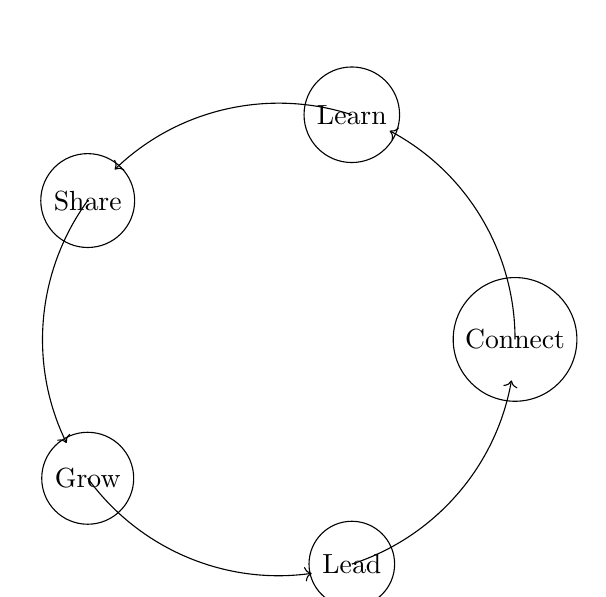
\begin{tikzpicture}
        % Community engagement cycle
        \foreach \angle/\label in {
            0/Connect,
            72/Learn,
            144/Share,
            216/Grow,
            288/Lead
        } {
            \node[draw,circle] at (\angle:3) {\label};
            \draw[->] (\angle:3) arc (\angle:\angle+62:3);
        }
    \end{tikzpicture}
    \caption{Community Engagement Cycle}
\end{figure}


\section{Resource Access Guide}
\begin{tcolorbox}[colback=white,colframe=primary,title=\textbf{Digital Resources}]
    \begin{enumerate}
        \item Document Templates
        \item Market Research
        \item Expert Directory
        \item Event Calendar
        \item Discussion Forums
        \item Knowledge Base
    \end{enumerate}
\end{tcolorbox}


\section{Community Benefits}
\begin{center}
    \begin{tabular}{p{0.3\textwidth}|p{0.6\textwidth}}
        \textbf{Benefit}    & \textbf{Description}                  \\
        \hline
        Expert Access       & Direct connection to industry experts \\
        Resource Library    & Comprehensive template collection     \\
        Market Intelligence & Regular market updates and analysis   \\
        Networking          & Regular virtual and physical events   \\
        Support             & Dedicated community support team      \\
    \end{tabular}
\end{center}

\begin{importantbox}
    Visit circle.counseal.com to activate your membership and access these resources.
\end{importantbox}

\end{document}